\documentclass[swedish,a4paper]{article}
\usepackage[swedish]{babel}
\usepackage[utf8]{inputenc}
\usepackage{amsmath}
\usepackage{amssymb}
\usepackage{csquotes} % Recommended
\usepackage{graphicx}
\usepackage{caption}
\usepackage[titletoc]{appendix}
\usepackage{listings, listings-rust}
\usepackage{longtable}
\usepackage{tikz}
\usepackage{tikz-cd}
\usepackage[nopostdot,nonumberlist]{glossaries}
\usepackage{pgfplots}
\usepackage{color}
\usepackage[margin=2cm]{geometry}
\usepackage[
style=authoryear,
sorting=nty,
backend=biber, 
natbib=true]{biblatex}

\usepackage{hyperref}
\usepackage[swedish]{cleveref}
\usepackage{adjustbox}
\usepackage{float}
% \overfullrule=5pt % diognosing overflow, draws an black line 

\makeglossaries
\glstoctrue
\newglossaryentry{enarray}{
  name=array,
  description={En serie av värdena, där varje värde kallas för element}
}

\newglossaryentry{2darray}{
  name=tvådimensionell array,
  description={En indexerad samling av data i en serie}
}

\newglossaryentry{matris}{
  name=matris,
  description={Data i två dimensioner som en tabell}
}

\pgfplotsset{compat=1.14}
\lstset{ % General settings for listings
basicstyle=\ttfamily\small, 
commentstyle=\color{green},
keywordstyle=\color{blue},
stringstyle=\color{red},
tabsize=4,
showstringspaces=false,
breaklines=true
}

% Redefine the listing name after loading cleveref
% \renewcommand{\lstlistingname}{Kodlistning}
% \crefname{lstinputlisting}{kodlistning}{kodlistningar} % For cleveref, singular and plural
% \Crefname{lstinputlisting}{Kodlistning}{Kodlistningar} % For cleveref, singular and plural, capitalized

\addbibresource{references.bib}
\renewcommand{\appendixpagename}{Bilagor}
\renewcommand*{\bibfont}{\small} % Adjust font size
\setlength{\bibitemsep}{1.5em} % Increase space between entries
\setlength{\bibhang}{2em} % Indent bibliography entries

\title{Vet inte än DEN kula TITLEN}
\author{Leo Altebro & Eduards Abisevs}
% \date{ }

\renewcommand*\contentsname{Innehåll}



\begin{document}
\begin{titlepage}
	\begin{minipage}[t]{0.45\textwidth}
		\raggedright
		NTI Gymnasiet - Nacka Strand \\
		Teknikprogrammet-Teknikvetenskap \\
		Gymnasiearbete 100p \\
		HT 2023 - VT 2024
	\end{minipage}
	% \hfill
	\begin{minipage}[t]{0.5\textwidth}
		\raggedleft
		\begin{adjustbox}{valign=t}
			
\includegraphics[width=\linewidth]{images/logo.jpg}
		\end{adjustbox}
	\end{minipage}

	\vspace*{\fill} % Add vertical space to center the title

	\begin{center}
		\Large\textbf{En ny potentiell automatiskt kortleksblandare}\\
		\large\textit{Proof of Concept av en kortblandare}
	\end{center}

	\vspace*{\fill} % Add vertical space to center the title

	\begin{minipage}[b]{0.45\textwidth}
		\raggedright
		Namn: Eduards Abisevs\\
		E-post: eduards.abisevs@elev.ga.ntig.se\\
		Namn: Leo Altebro\\
		E-post: leo.altebro@elev.ga.ntig.se\\
		Handledare: Elias
	\end{minipage}
	\begin{minipage}[b]{0.5\textwidth}
		\raggedleft
		Typsatt med \LaTeX. \\
		Kompilerad \today.
	\end{minipage}
\end{titlepage}

% \maketitle

\tableofcontents
\newpage

\section{Inledning}
\subsection{Introduktion till ämnet}
Spelbranschen är en industri som omsätter miljardbelopp och precis som alla
industrier utvecklas den med resten av världen. Industrier över hela världen har
som mål att hitta nya sätt att effektivisera och sänka kostnad på det arbete som
utförs för att bedriva vinst och spelbranschen har följt denna långvariga trend
med till exempel online casinon. Inom spelbranschen är kortspel vanligt
förekommande, att försöka automatisera dem är ett logiskt steg att ta, men för
en så stor industri vill man vara extra säker på att allt utförs på bästa sätt.
Alla sätt att blanda kort är nämligen inte lika bra, vilken sorteringsmetod som
används kan ha påverkan på resultatet. Teknologins inflytande inom spelbranschen
ökar kraftigt, de största delarna av branschen bedrivs mer och mer av maskiner
och algoritmer som får stor potentiellt inflytande på spelresultat, därför är
det bäst att börja tänka på möjliga problem så snart som möjligt. Redan nu finns
det blandningsmaskiner för kortlekar som vi inte vet någonting om; varken hur de
funkar eller hur bra de är. Allt som vi vet är de är certifierade av
tredjepartsföretag. Faktumet att de kan kosta upp till 100 000 kr betyder att
inte vem som helst kan ha tillgång till en kortblandningsmaskin.

\subsection{Syfte}

Syftet med denna undersökning är att ta fram den hypotetiskt bästa kortblandaren
utifrån två faktorer: 1) hur slumpmässigt den algoritm som den byggs efter kan
blanda kort; 2) till vilken grad den potentiella maskinen byggd efter algoritmen
skulle fungera i verkligheten. Med resultaten förväntas variationen i
slumpmässighet för olika blandningsmetoder kunna visas upp samt kunna använda de
resultaten för att komma fram till den hypotetiskt definitiva maskinen, något
som är viktigt då spelbranschen handlar mycket om chans. Det är därför viktigt
att se till så allt funkar på bästa sätt. I den här vetenskapliga rapporten
kommer en jämförelse av hur effektivt framtagna blandningsmetoder kan fungera i
en hypotetisk blandningsmaskin att utföras. Samtidigt som man kan utforska hur
en dator kan göra slumpmässiga sekvenser på ett effektivt sätt med tanken att
den ska tillämpas till en potentiell kortblandare. Detta är viktigt för att
spelbranschen är en stor industri som handlar mycket om tur, att se till att de
slumpmässiga resultaten är framtagna på bästa möjliga sätt är en essentiell del.
Vi söker med hjälp av data svaret på frågan:

Utifrån slumpmässighet och effektivitet, vilken kort blandningsmetod är bäst för
en potentiell spelkortsblandare som uppfyller följande:
\begin{itemize}
	\item Fysiskt tillämpning: Hur pass väl den kan framställas i verkligheten 
	\item Effektivet: Utifrån mjukvaras och hårdvaras perspektiv
        \item Kortblandnings slumpmässighet
\end{itemize}


\section{Teori}
\subsection{Beräkningsteori}

Beräkningsteori är en del av matematik vars syfte är grundat i hur och om
problem kan bli lösta på olika beräkningssätt. Beräkningsteori har flera olika
grenar. En gren handlar om vad som går att bevisa inom matematik angående om
nummer och funktioner är beräknelig eller inte. Med beräknelig menas något som
kan beräknas, det vill säga värderas, uppfattas eller förutses, när det kommer
till matematik syftar det på att bestämma något via matematiska
modeller/processer, alltså att kalkylera.

\subsection{Slumpmässighet}

Slumpmässighet är en egenskap som anger att något sker utan klart mönster, när
något är helt slumpmässigt är det i princip omöjligt att förutse. Slumpmässighet
inom matematik är byggd beräknings\-teori och den delas upp i två beroende på om
det gäller slumpmässighet av en bestämd mängd eller en oändlig mängd av objekt
\parencite{Terwijn2016}.

\subsection{Algoritmer}
Theoretical Whats and whys  angående algorithmer

\subsubsection{Pile shuffle}
\label{sec:pile_shuffle}
Pile shuffle är en typ av kortleksblandings metod som genomförs med fysiska kort. Processen utgår att ett kort
från kortleken läggs i en av högar. Processen försätts tills alla kort från kortleken är i sina högar. Sedan läggs ihop alla högar i ett nytt kortlek. 


\begin{figure}[ht]
	\begin{center}
		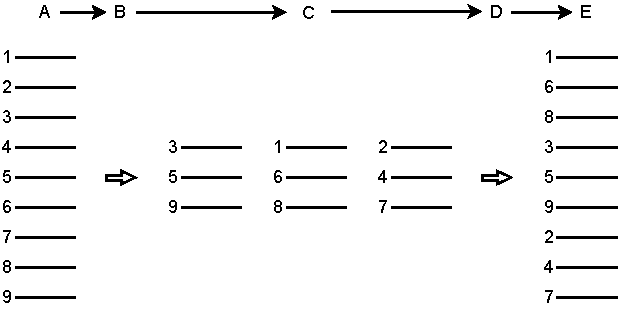
\includegraphics{images/pile_shuffle.pdf}
	\end{center}
	\captionsetup{justification=centering,margin=4cm}
	\caption{Steg i processen för Pile Shuffle. Illustrationen visar de
	iterativa stegen från den ursprungliga högen (A), genom uppdelning i
	högar (B), temporara högar (C), omarrangering av temporara högar (D),
	och tillbaka till en enda hög (E). Pilar indikerar riktningen för
	blandningsprocessen.
	}
	\label{fig:pile_shuffle_1}
\end{figure}

\subsubsection{Riffle shuffle}
Mest kända kortleksblandings metoden som har undersökets under många tiotals år.


\subsection{Klassiskt poker test}
\label{sec:poker_test}
Ett klassiskt poker test används att avgöra slump\-mässighet i numeriska 
sekvenser, oftast för att testa slumptalsgeneratorer. Testet utförs genom
att 3 till 5 nummer väljs ut ur en sekvens och placeras i en av sju  kategorier beroende på mönstret som talen har, mönsterna är baserade på händer i poker vilket är varför testet kallas poker test \parencite{Abdel2014}. 
Det olika mönster som letas efter i talen visas i \cref{tab:num_poker_hands}.

\begin{table}[h] % h as i here, place it here (as in source code!)
	\centering
	\begin{tabular}{|l|c|}
	\hline 
	Pokerhand & Mönster \\ \hline  
	Femtal & AAAAA \\ \hline
	Fyrtal & AAAAB \\ \hline
	Kåk & AAABB \\ \hline
	Tretal & AAABC \\ \hline
	Tvåpar & AABBC \\ \hline
	Par & AABCD \\ \hline
	Högt kort & ABCDE \\ \hline
	
\end{tabular}
\caption{Vanliga kategorier till poker test}
\label{tab:num_poker_hands}
\end{table}

 Antalet mönster i varje kategori räknas för att få en distribution, som
 då jämförs med en distribution som stämmer överens med sannolikheten
 att få dem olika mönster. Om det total antalet mönster är $n$ och
 sanolikheten för en pokerhand $i$ är $p_i$, så borde antalet mönster i
 den kategori vara $$o_i = p_i * n$$ Där $o_i$ är antalet mönster som
 borde matcha pokerhand $i$. För att bestäma om resultaten kan komma
 från en rättvis kortlek så jämnförs de resultat som fåtts av att plocka
 ut nummer mot de resultat som fås av sannolikhet via ett chi-två-test.

\begin{equation*}
\end{equation*}

\subsubsection{Chi-två-test}
\label{sec:chi_square}
Inom statistik används ett \textit{goodness-of-fit} test för att mäta
hur pass väl fördelningen för den data som observerats stämmer överens
med fördelningen som data förväntas ha utifrån en model. Karl Pearsons
chi-två-test kan användas som \textit{goodness-of-fit} test, det
använder chitvåfördeling. I testet jämnförs ett värde $\chi^2$ med ett
kritiskt värde för att bestäma om den observerade följer den förväntade
fördelningen. $\chi^2$ beräknas enligt formlen $$ \chi^2 = \sum_{i=1}^k
\frac{(O_i - E_i)^2}{E_i}$$ Där $O_i$ är observerade frekvensen för en
kategori av data $i$ och $E_i$ är förväntade frekvensen för kategorin
$i$ \parencite{nist}. Det kritiska värdet fås av antalet
frihetsgrader(kategorier - parametrar) och signifikansnivån som bestämts
för testet.


%Chi-square, chi-två testing eller som den också betecknas $\chi^2$ är statistikt test
%som oftas används till att definera och beräkna slumpmässighet av bestämd sannolikhet.
%$$ \chi^2 = \sum_{i=1}^k \frac{(O_i - E_i)^2}{E_i}$$
%Vart $O_i$ är observerade frekvensen för kategorin $i$ och $E_i$ är förväntade
%frekvensen för kategorin $i$ \parencite{nist}.

\subsection{Pseudoslumptalsgenerator (PRNG)}
Här berätta om ChaCha20 \parencite{chacha} den som är biobliotekes rand
\parencite{rand_crate} default PRNG och mersenne twister som egentligen var första
hands val
\parencite{mersenne_twister} men som vi sedan bytte till ChaCha för att i rust
är det relativt svårt att  implementera och använda mersenne twister. Berätta om
dem skillnaderna som finns.


En väldigt känd och testad algoritm är Mersenne Twister (MT 19937) som
har en väldigt långt period innan siffrorna börjar att upprepa sig, mer
exakt $2^{19937}$ \parencite{mersenne_twister}.

Alltså nämn att för att det här är som et proof of concept, borde vid
senare tillfälle användas en hårdvara PRNG och icke software PRNG.
Men på grund av detta undersökning handlar mesta dels om stora mängder av data
simulationer så måste vi använda och "Sacrifice" verkliga till att lättare
skapa simulationer!

\section{Metod} 
Metoden kan indelas i tre huvudområderna
1) framtagande av algoritmerna. 
2) simulation av kortlkesblandningar. 
3) statistiska tester av rådata.
Målet är att besvara en av frågestälningens kriterium "Kortblandnings
slumpmässighet ". Därför valdes det att utföra ett kvantitiv undersökning med
hjälp av simulation och statistiska tester. Simulation valdes till för
att generera stora mängder av kortlkesblandningar med målet att
simulationen (processmässight) skulle vara snarlik ett fysiskt
kortleks\-blandare under sin livscykel. 
% dvs på liknande sätt hur ett fysiskt kortleks\-blandare skulle används under dens livscykel. 



\subsection{Testmiljö} 
\begin{table}[ht]
\centering
\begin{tabular}{|l|p{7cm}|} 
\hline
Typ & Specification  \\ \hline
Processor & AMD Ryzen 5 3600 \newline 6 cores / 12 threads \newline 3.6 GHz \\ \hline
RAM & 15.93 GB \\ \hline
Hårdisk & KINGSTON SA400S3, 447 GB \\ \hline
Operativsystem & \texttt{Ubuntu 22.04.3 (LTS) x86\_64, \newline Linux kernel 6.2.0-36-generic} \\ \hline
\end{tabular}
\caption{Linux Dator}
\label{tab:linux_env}
\end{table}
I valet av testmiljö prioriterades operativsystemets kompatabilitet av
dem utvecklingsverktyg som användes. Linux valdes på grund av dess
robusta stöd för programmeringsmiljöer och bred stöd för
mjukvaruutvecklingsverktyg. Dessutom erbjuder Linux bättre kontroll
över systems\-resurer. Vilket är avgörande för att uppnå följdriktiga
och till\-för\-litliga testresulat. Därför kördes undersökningen på en
Linux dator med specifikationerna listade i tabell \ref{tab:linux_env}.

% Datan insamlades från digitalt simulation på olika kortblandningsmetoder
% i Rust version 1.73. De algoritmerna som undersöktes var skrivna i
% programspråk Rust i försök att göra dem så likt verkligheten som
% möjligt. 

% För statistikst analys av data användes programmeringsspråket Python
% 3.11 och utnyttjades bibliotek som Numpy till datamängd bearbetning,
% Scipy till statistisk analys och Matplotlib till visualisering av
% resultat. 


\subsection{Simulation för kortblandningar och implementation}
Simulation och blandnings algoritmerna implementerades i programmerings
språk Rust. Rust är ett programmeringsspråk som fokuserar på
minnessäkerhet, parallellism och minneseffektivitet. Rust är känt för
sina avancerade funktioner som ägarskapssystemet (ownership), vilket
hjälper till att förhindra minnesläckor och tillåter säker
minneshantering utan en skräpsamlare (garbage collector)
\parencite{rust}. Detta har ökad populäritet i användning av Rust i
inbyggda system som ett motkandidat till c/c++. 
%Rådata ifrån simulationer sparades. Sedan lästes in i Python program.  

Programmet utvecklades med Rust version 1.73.0 och användes bibliotek
(Rust Crates) som Rand version 0.8 för PRNG \parencite{rand_crate}.
Rayon för enkel användning av  parallell multiprocessing
\parencite{rayon_crate}. Simulation utgår från att man genererar
tvådimmensionella array, detta kan matematikst beskrivas som matris med
bestämd mängd av kortlekar. Vart varje kort, låt kalla dem till $x$ som
följer följande mängden $\{x \in \mathbb{N},  0 \leq x \leq 51 \}$
Resulterande datamängden är en \gls{matris} $D$ med 52 kolumner och $m$ antal
rader, vart $m$ värde visar hur många kortlekar det finns i datamängden.

\begin{equation*}
	D = \begin{bmatrix}
		x_{0,0} & x_{0,1} & x_{0,2} & \cdots & x_{0,51}\\ 
		x_{1,0} & x_{1,1} & x_{1,2} & \cdots & x_{1,51}\\
		x_{2,0} & x_{2,1} & x_{2,2} & \cdots & x_{2,51}\\
		\vdots & \vdots & \vdots & \; & \vdots \\
		x_{m,0} & x_{m,1} & x_{m,2} & \cdots & x_{m,51}
	\end{bmatrix}
\end{equation*}

För att bestämma $m$ värde följdes ett kriterium från ett av testerna som ska
utföras, klassiskt poker test mer i  detalj beskriven i underrubriken
\ref{sec:chi_square} . Till hjälps användes \parencite{nist} internätkälla, i
denna nämns det att det är viktigt för chi-square approximationens trovärdighet
att minsta kategorin ska inte vara mindre än fem teoretiska framkommande i den
kategorin. Detta ska tillämpas till simulationen på följande sätt. Det är
viktigt att hitta den minsta kategorin som kan förekomma. I poker är den mest
sällsynta pokerhand kungliga färgstege (Royal Flush) som kan räknas ut på
följande sätt antal av alla kortkombinationer med fem kort. $\binom{52}{5} =
2\,598\,960$ Kungliga färgstege finns det fyra  kombinationer av i kortleken
som kan räknas ut på följande sätt totala antal kombinationer av kungliga
färgstege delat med totala antal femkorts kombinationer från standardkortlek.
$$ P(\text{Kunglig färgstege}) =  \frac{\binom{4}{1}}{\binom{52}{5}} =
\frac{4}{2\,598\,960} \approx \frac{1}{649\,740} $$ $$m = P(\text{Kunglig
färgstege})  \times 5 = 3\,248\,700$$ detta blir den minimala datamängden i simulationen
.

\subsubsection{Val av datatyp \& rådatalagring} Efter teoretiska beräkningar av
datamängden är det viktigt att välja lämplig datatyp att representera data i.
Högsta talet som behövs är 51 definerad tidigare och betecknat med $x$. Detta
betyder att minsta datatypen får användas som är 8 bit eller 1 byte långa som
kan  innehålla följande värden $$\{b \in \mathbb{N},  0 \leq b \leq 255 \}$$ som
överns\-stämmer med datamängdens högsta talet $x$. Detta ger möjligheten att
använda den  fundermantala datatypen som används i minnes adressen. Fördelen med
detta är det simplifierar lagring och inmatning av datamängder i t.ex Python
med NumPy.

Andra aspekten till varför datatypen är viktigt är att spara minnen för att det
kommer att simuleras och sparas tiotals rådata filer varje fil kommer att väga
$161 MB$,
detta kan räknas ut på följande sätt
$$ \frac{\text{totala bytes}}{\text{megabyte (MB)}} = \frac{52 \times m }{1024 \times
1024} = \frac{52 \times 3\,248\,700}{1024 \times 1024} = \frac{168\,932\,400}{1\,048\,576} \approx 161 MB 
$$
som det är enkelt att spara data i binärt format för att 8 bits eller 1 byte
är en fundamental och uniform mått i minnesadressen. Med det sagt ingen data
bearbetning behövs och det är enkelt att ladda in denna i till exempel Python
med numpy till statistiska testerna av rådata

Därför att sista teoretiska delen att bestämma
är hur många iterationer per algoritm ska genomföras. Med iterationer menas
hur många gånger kortleken blandas följande på varandra.

\subsection{Kortblandings algoritmernas implemenation}

Då tanken var att  algoritmerna skulle potentiellt användas i ett fysiskt
inbäddad system fanns det vissa  kriterier som algoritmerna skulle följa: det
skulle gå att bygga en maskin, den skulle vara slumpmässig, dvs. simulation

\subsubsection{Riffle shuffle}
Det här är riffle shuffle, vi ska nu parata om detta närmare...
så funkar det här då?? Yeeep det gör det $\binom{55}{2} = \theta$

\subsubsection{Implementation av Pile shuffle}
Inspiration att undersöka pile shuffle kom ifrån \textcite{3DprintedLife2021},
där pile shuffle implementerades i en 3d printat kortleksblandare.  

\subsection{statistiska tester}
Statistiska tester utfördes med Python version 3.11. Python är en
objektorienterad, dynamiskt typad programmerings språk med fokus på
läsbarhet \parencite{python}. Python används ofta i statiskt analys på
grund av dens läsbarhet och lätt använding därför finns det många
avancerade bibliotek (samling av färdig kod) till numerisk analys som
NumPy som är snabbt i vektoriserad aritmetik och SciPy som har många
inbygga statistiska tester som $\chi^2$-testet \parencite{numpy, scipy}.
Därför valdes det att utföra statistika tester som Poker test och
StdMean testet i Python 3. Pga att avgörande av slumpmässighet är domän
specifikt och rent matematiskt komplex som kräver högre förstålse i
matematiska området inom statistiska. Därför valdes det bort att utföra
metoder som entropi, ApEn \parencite{ApEn}. Från andra sidan är
simulation enklare att utföra och analysera data med avseende på
förväntade frekvensen ($\chi^2$-testet) samt enklare statistiska koncept
som mediana och standardavviklse (StdMean-testet).    

% För statistikst analys av data användes programmeringsspråket Python
% 3.11 och utnyttjades bibliotek som Numpy till datamängd bearbetning,
% Scipy till statistisk analys och Matplotlib till visualisering av
% resultat. 

Rådata som sparades efter simulationen är laddat in som en dimensionell
\gls{enarray} med hjälp av Numpy  efter det är rådata återställt tillbaka till
tvådimensionell matris för vidare bearbetning och analys med följande
metoder: Klassisk Poker Test \ref{sec:poker_test} och medelvärde av
korta positioner i kortleken över hela datamängden kalkylerad såsom
avvikelser av dessa positioner. Utförligt beskrivning i underrubriker. 

\subsubsection{implemention av Klassiskt poker test}
Poker Test utgår ifrån att man karaktäriserar typer av mönster till 
pokerhänder och kalkylerar  den absolutvärdet $\chi^2$ i detalj beskrevs
teorin bakom $\chi^2$ testet i sektion
\ref{sec:poker_test}. 

\subsubsection*{Kategorisering}
I standardkortlek finns det 52 kort med fyra olika 
färger (Spader, Hjärter, Ruter och klöver) och 13 valörer 
(2, 3, 4, 5, 6, 7, 8, 9, 10, Knekt, Dam, Kung, Ess).
Av skall att testerna utförs med standard kortleken,

\begin{table}[ht] 
\captionsetup{justification=centering,margin=4cm}
\caption{Alla pokerhänders namn, relativt mönster och antal av kombinationer }
\label{tab:all_poker_hands}
	\centering
	\begin{tabular}{|l|c|r|}
	
	% Header
	\hline 
	Pokerhand 
	& Example på mönster 
	& Antal kombinationer 
	\\ \hline  

	% rows
	Kunglig färgstege 
	& $A\spadesuit\, K\spadesuit\, Q\spadesuit\, J\spadesuit\, 10\spadesuit$
	& 4 
	\\ \hline

	Färgstege
	& $K\spadesuit\, Q\spadesuit\, J\spadesuit\, 10\spadesuit\, 9\spadesuit$
	& 36 
	\\ \hline

	Fyrtal 
	& $A\spadesuit\,A\heartsuit\,A\diamondsuit\,A\clubsuit\, K\spadesuit$ 
	& 624 
	\\ \hline

	Kåk 
	& $A\spadesuit\, A\heartsuit\, A\diamondsuit\, K\clubsuit\,K\spadesuit$ 
	& 3\,744
	\\ \hline

	Färg
	& $K\spadesuit\, Q\spadesuit\, J\spadesuit, 10\spadesuit\, 8\spadesuit$
	& 5\,108
	\\ \hline

	Stege 
	& $K\spadesuit\, Q\heartsuit\, J\diamondsuit\, 10\clubsuit\,9\spadesuit$ 
	& 10\,200
	\\ \hline
	Triss 
	& $A\spadesuit\, A\heartsuit\, A\diamondsuit\, K\clubsuit\, Q\spadesuit$
	& 54\,912
	\\ \hline

	Två par 
	& $A\spadesuit\, A\heartsuit\, K\diamondsuit\, K\clubsuit\, Q\spadesuit$
	& 123\,552
	\\ \hline

	Ett par 
	& $A\spadesuit\, A\heartsuit, K\diamondsuit\, Q\clubsuit\, J\spadesuit$ 
	& 1\,098\,240 
	\\ \hline

	Högt kort
	& $A\spadesuit\, Q\heartsuit\, J\diamondsuit\, 5\clubsuit\, 4\spadesuit$
	& 1\,302\,540
	\\ \hline

	 
	\multicolumn{2}{|r|}{Summan:} 
	& 2\,598\,960 
	\\ \hline
\end{tabular}
\end{table}

valdes det att anpassa $\chi^2$ testet att använda alla poker händer. Matematiken
speciellt kombinatoriken att räkna ut sannolikheter och frekvensen av alla poker\-
händer är relativt svårt uppdrag därför addopterdes det \textcite{Drew2006} 
uträkningar se tabell \ref{tab:all_poker_hands}. Detta medföljde med mer komplex
karakterisering av poker\-händer än när man använder $\chi^2$ testet 
att till example testa slumptalsgeneratorer. Valet log med att datamängderna 
innehåller kortlekar till att göra simulationer mer  realistiska och anpassade
till hur ett riktigt kortleksblandare skulle fungera i drift. Därför valet att
anpassa statistiska tester till slutmål användnings sätt verkade vara ett
logiskt steg att ta.

Poker Test kan anpassas till vilken som helst sekvens av nummer 3-5 stora
mängder. Men för att vår simulation använder vi samma nummer som pokerkort
därför kan vi anpassa klassiska poker test var man använder alla möjliga
pokerhänder av sekvens av 5 kort. Resultatet från karakterisering av händer
använder man i en chi-square testet. För att göra testet rätt följde jag
Engineering Statistics handbok (NIST 2012). Dvs för att avgöra hur många 
händer
uppkom med avseende till teoretiska värdena EXPECTED vs OBSERVED värdena. sen
jämför man chi-square resultatet till en CRITICAL värde om den värden som vi
fick är mindre kan vi med säkerhet säga att algoritmen är slumpmässigt och 
vice versa.

Testet utgår i två generella steg kategorisera fem kort och seden 

\subsubsection{Implemention av StdMean testet}
Datamängden är utformat på sätt att kort värde är alltså dess position i
kortleken. Första kort är 0 dvs position 0 i kortleken. Kalkylerar varje
columns korts medelvärde och standaravvikelse ska man förustpå att medelvärde
borde ligga nära $51/2= 25.5$ detta betyder att i position 0 har alla kort varit
i, och om standaravviklse i figuren är höga torn har position 0 stort variation
av vilka kort som var där. Detta är då en indikator på en uniform distribution
som betyder en slumpmässigt algoritm.

\section{Resulat}
Result är icke bestämt i vilken format kommer att skrivas
Men dem kommer att innehålla figur \ref{fig:test_figure}. Antagligen mest 
intresanta figurer kommer att visas här och alla andra Bilagas i Appendix.
För att det kommer att vara minst 30 figurer och chi två tabeller(dem 
kan göras i ett större tabel, antar jag)

\begin{figure}[ht]
    \begin{center}
        %% Creator: Matplotlib, PGF backend
%%
%% To include the figure in your LaTeX document, write
%%   \input{<filename>.pgf}
%%
%% Make sure the required packages are loaded in your preamble
%%   \usepackage{pgf}
%%
%% Also ensure that all the required font packages are loaded; for instance,
%% the lmodern package is sometimes necessary when using math font.
%%   \usepackage{lmodern}
%%
%% Figures using additional raster images can only be included by \input if
%% they are in the same directory as the main LaTeX file. For loading figures
%% from other directories you can use the `import` package
%%   \usepackage{import}
%%
%% and then include the figures with
%%   \import{<path to file>}{<filename>.pgf}
%%
%% Matplotlib used the following preamble
%%   \def\mathdefault#1{#1}
%%   \everymath=\expandafter{\the\everymath\displaystyle}
%%   
%%   \makeatletter\@ifpackageloaded{underscore}{}{\usepackage[strings]{underscore}}\makeatother
%%
\begingroup%
\makeatletter%
\begin{pgfpicture}%
\pgfpathrectangle{\pgfpointorigin}{\pgfqpoint{6.400000in}{4.800000in}}%
\pgfusepath{use as bounding box, clip}%
\begin{pgfscope}%
\pgfsetbuttcap%
\pgfsetmiterjoin%
\definecolor{currentfill}{rgb}{1.000000,1.000000,1.000000}%
\pgfsetfillcolor{currentfill}%
\pgfsetlinewidth{0.000000pt}%
\definecolor{currentstroke}{rgb}{1.000000,1.000000,1.000000}%
\pgfsetstrokecolor{currentstroke}%
\pgfsetdash{}{0pt}%
\pgfpathmoveto{\pgfqpoint{0.000000in}{0.000000in}}%
\pgfpathlineto{\pgfqpoint{6.400000in}{0.000000in}}%
\pgfpathlineto{\pgfqpoint{6.400000in}{4.800000in}}%
\pgfpathlineto{\pgfqpoint{0.000000in}{4.800000in}}%
\pgfpathlineto{\pgfqpoint{0.000000in}{0.000000in}}%
\pgfpathclose%
\pgfusepath{fill}%
\end{pgfscope}%
\begin{pgfscope}%
\pgfsetbuttcap%
\pgfsetmiterjoin%
\definecolor{currentfill}{rgb}{1.000000,1.000000,1.000000}%
\pgfsetfillcolor{currentfill}%
\pgfsetlinewidth{0.000000pt}%
\definecolor{currentstroke}{rgb}{0.000000,0.000000,0.000000}%
\pgfsetstrokecolor{currentstroke}%
\pgfsetstrokeopacity{0.000000}%
\pgfsetdash{}{0pt}%
\pgfpathmoveto{\pgfqpoint{0.800000in}{0.528000in}}%
\pgfpathlineto{\pgfqpoint{5.760000in}{0.528000in}}%
\pgfpathlineto{\pgfqpoint{5.760000in}{4.224000in}}%
\pgfpathlineto{\pgfqpoint{0.800000in}{4.224000in}}%
\pgfpathlineto{\pgfqpoint{0.800000in}{0.528000in}}%
\pgfpathclose%
\pgfusepath{fill}%
\end{pgfscope}%
\begin{pgfscope}%
\pgfsetbuttcap%
\pgfsetroundjoin%
\definecolor{currentfill}{rgb}{0.000000,0.000000,0.000000}%
\pgfsetfillcolor{currentfill}%
\pgfsetlinewidth{0.803000pt}%
\definecolor{currentstroke}{rgb}{0.000000,0.000000,0.000000}%
\pgfsetstrokecolor{currentstroke}%
\pgfsetdash{}{0pt}%
\pgfsys@defobject{currentmarker}{\pgfqpoint{0.000000in}{-0.048611in}}{\pgfqpoint{0.000000in}{0.000000in}}{%
\pgfpathmoveto{\pgfqpoint{0.000000in}{0.000000in}}%
\pgfpathlineto{\pgfqpoint{0.000000in}{-0.048611in}}%
\pgfusepath{stroke,fill}%
}%
\begin{pgfscope}%
\pgfsys@transformshift{1.025455in}{0.528000in}%
\pgfsys@useobject{currentmarker}{}%
\end{pgfscope}%
\end{pgfscope}%
\begin{pgfscope}%
\definecolor{textcolor}{rgb}{0.000000,0.000000,0.000000}%
\pgfsetstrokecolor{textcolor}%
\pgfsetfillcolor{textcolor}%
\pgftext[x=1.025455in,y=0.430778in,,top]{\color{textcolor}{\rmfamily\fontsize{10.000000}{12.000000}\selectfont\catcode`\^=\active\def^{\ifmmode\sp\else\^{}\fi}\catcode`\%=\active\def%{\%}$\mathdefault{0}$}}%
\end{pgfscope}%
\begin{pgfscope}%
\pgfsetbuttcap%
\pgfsetroundjoin%
\definecolor{currentfill}{rgb}{0.000000,0.000000,0.000000}%
\pgfsetfillcolor{currentfill}%
\pgfsetlinewidth{0.803000pt}%
\definecolor{currentstroke}{rgb}{0.000000,0.000000,0.000000}%
\pgfsetstrokecolor{currentstroke}%
\pgfsetdash{}{0pt}%
\pgfsys@defobject{currentmarker}{\pgfqpoint{0.000000in}{-0.048611in}}{\pgfqpoint{0.000000in}{0.000000in}}{%
\pgfpathmoveto{\pgfqpoint{0.000000in}{0.000000in}}%
\pgfpathlineto{\pgfqpoint{0.000000in}{-0.048611in}}%
\pgfusepath{stroke,fill}%
}%
\begin{pgfscope}%
\pgfsys@transformshift{1.909590in}{0.528000in}%
\pgfsys@useobject{currentmarker}{}%
\end{pgfscope}%
\end{pgfscope}%
\begin{pgfscope}%
\definecolor{textcolor}{rgb}{0.000000,0.000000,0.000000}%
\pgfsetstrokecolor{textcolor}%
\pgfsetfillcolor{textcolor}%
\pgftext[x=1.909590in,y=0.430778in,,top]{\color{textcolor}{\rmfamily\fontsize{10.000000}{12.000000}\selectfont\catcode`\^=\active\def^{\ifmmode\sp\else\^{}\fi}\catcode`\%=\active\def%{\%}$\mathdefault{10}$}}%
\end{pgfscope}%
\begin{pgfscope}%
\pgfsetbuttcap%
\pgfsetroundjoin%
\definecolor{currentfill}{rgb}{0.000000,0.000000,0.000000}%
\pgfsetfillcolor{currentfill}%
\pgfsetlinewidth{0.803000pt}%
\definecolor{currentstroke}{rgb}{0.000000,0.000000,0.000000}%
\pgfsetstrokecolor{currentstroke}%
\pgfsetdash{}{0pt}%
\pgfsys@defobject{currentmarker}{\pgfqpoint{0.000000in}{-0.048611in}}{\pgfqpoint{0.000000in}{0.000000in}}{%
\pgfpathmoveto{\pgfqpoint{0.000000in}{0.000000in}}%
\pgfpathlineto{\pgfqpoint{0.000000in}{-0.048611in}}%
\pgfusepath{stroke,fill}%
}%
\begin{pgfscope}%
\pgfsys@transformshift{2.793725in}{0.528000in}%
\pgfsys@useobject{currentmarker}{}%
\end{pgfscope}%
\end{pgfscope}%
\begin{pgfscope}%
\definecolor{textcolor}{rgb}{0.000000,0.000000,0.000000}%
\pgfsetstrokecolor{textcolor}%
\pgfsetfillcolor{textcolor}%
\pgftext[x=2.793725in,y=0.430778in,,top]{\color{textcolor}{\rmfamily\fontsize{10.000000}{12.000000}\selectfont\catcode`\^=\active\def^{\ifmmode\sp\else\^{}\fi}\catcode`\%=\active\def%{\%}$\mathdefault{20}$}}%
\end{pgfscope}%
\begin{pgfscope}%
\pgfsetbuttcap%
\pgfsetroundjoin%
\definecolor{currentfill}{rgb}{0.000000,0.000000,0.000000}%
\pgfsetfillcolor{currentfill}%
\pgfsetlinewidth{0.803000pt}%
\definecolor{currentstroke}{rgb}{0.000000,0.000000,0.000000}%
\pgfsetstrokecolor{currentstroke}%
\pgfsetdash{}{0pt}%
\pgfsys@defobject{currentmarker}{\pgfqpoint{0.000000in}{-0.048611in}}{\pgfqpoint{0.000000in}{0.000000in}}{%
\pgfpathmoveto{\pgfqpoint{0.000000in}{0.000000in}}%
\pgfpathlineto{\pgfqpoint{0.000000in}{-0.048611in}}%
\pgfusepath{stroke,fill}%
}%
\begin{pgfscope}%
\pgfsys@transformshift{3.677861in}{0.528000in}%
\pgfsys@useobject{currentmarker}{}%
\end{pgfscope}%
\end{pgfscope}%
\begin{pgfscope}%
\definecolor{textcolor}{rgb}{0.000000,0.000000,0.000000}%
\pgfsetstrokecolor{textcolor}%
\pgfsetfillcolor{textcolor}%
\pgftext[x=3.677861in,y=0.430778in,,top]{\color{textcolor}{\rmfamily\fontsize{10.000000}{12.000000}\selectfont\catcode`\^=\active\def^{\ifmmode\sp\else\^{}\fi}\catcode`\%=\active\def%{\%}$\mathdefault{30}$}}%
\end{pgfscope}%
\begin{pgfscope}%
\pgfsetbuttcap%
\pgfsetroundjoin%
\definecolor{currentfill}{rgb}{0.000000,0.000000,0.000000}%
\pgfsetfillcolor{currentfill}%
\pgfsetlinewidth{0.803000pt}%
\definecolor{currentstroke}{rgb}{0.000000,0.000000,0.000000}%
\pgfsetstrokecolor{currentstroke}%
\pgfsetdash{}{0pt}%
\pgfsys@defobject{currentmarker}{\pgfqpoint{0.000000in}{-0.048611in}}{\pgfqpoint{0.000000in}{0.000000in}}{%
\pgfpathmoveto{\pgfqpoint{0.000000in}{0.000000in}}%
\pgfpathlineto{\pgfqpoint{0.000000in}{-0.048611in}}%
\pgfusepath{stroke,fill}%
}%
\begin{pgfscope}%
\pgfsys@transformshift{4.561996in}{0.528000in}%
\pgfsys@useobject{currentmarker}{}%
\end{pgfscope}%
\end{pgfscope}%
\begin{pgfscope}%
\definecolor{textcolor}{rgb}{0.000000,0.000000,0.000000}%
\pgfsetstrokecolor{textcolor}%
\pgfsetfillcolor{textcolor}%
\pgftext[x=4.561996in,y=0.430778in,,top]{\color{textcolor}{\rmfamily\fontsize{10.000000}{12.000000}\selectfont\catcode`\^=\active\def^{\ifmmode\sp\else\^{}\fi}\catcode`\%=\active\def%{\%}$\mathdefault{40}$}}%
\end{pgfscope}%
\begin{pgfscope}%
\pgfsetbuttcap%
\pgfsetroundjoin%
\definecolor{currentfill}{rgb}{0.000000,0.000000,0.000000}%
\pgfsetfillcolor{currentfill}%
\pgfsetlinewidth{0.803000pt}%
\definecolor{currentstroke}{rgb}{0.000000,0.000000,0.000000}%
\pgfsetstrokecolor{currentstroke}%
\pgfsetdash{}{0pt}%
\pgfsys@defobject{currentmarker}{\pgfqpoint{0.000000in}{-0.048611in}}{\pgfqpoint{0.000000in}{0.000000in}}{%
\pgfpathmoveto{\pgfqpoint{0.000000in}{0.000000in}}%
\pgfpathlineto{\pgfqpoint{0.000000in}{-0.048611in}}%
\pgfusepath{stroke,fill}%
}%
\begin{pgfscope}%
\pgfsys@transformshift{5.446132in}{0.528000in}%
\pgfsys@useobject{currentmarker}{}%
\end{pgfscope}%
\end{pgfscope}%
\begin{pgfscope}%
\definecolor{textcolor}{rgb}{0.000000,0.000000,0.000000}%
\pgfsetstrokecolor{textcolor}%
\pgfsetfillcolor{textcolor}%
\pgftext[x=5.446132in,y=0.430778in,,top]{\color{textcolor}{\rmfamily\fontsize{10.000000}{12.000000}\selectfont\catcode`\^=\active\def^{\ifmmode\sp\else\^{}\fi}\catcode`\%=\active\def%{\%}$\mathdefault{50}$}}%
\end{pgfscope}%
\begin{pgfscope}%
\definecolor{textcolor}{rgb}{0.000000,0.000000,0.000000}%
\pgfsetstrokecolor{textcolor}%
\pgfsetfillcolor{textcolor}%
\pgftext[x=3.280000in,y=0.251766in,,top]{\color{textcolor}{\rmfamily\fontsize{10.000000}{12.000000}\selectfont\catcode`\^=\active\def^{\ifmmode\sp\else\^{}\fi}\catcode`\%=\active\def%{\%}Korts position}}%
\end{pgfscope}%
\begin{pgfscope}%
\pgfsetbuttcap%
\pgfsetroundjoin%
\definecolor{currentfill}{rgb}{0.000000,0.000000,0.000000}%
\pgfsetfillcolor{currentfill}%
\pgfsetlinewidth{0.803000pt}%
\definecolor{currentstroke}{rgb}{0.000000,0.000000,0.000000}%
\pgfsetstrokecolor{currentstroke}%
\pgfsetdash{}{0pt}%
\pgfsys@defobject{currentmarker}{\pgfqpoint{-0.048611in}{0.000000in}}{\pgfqpoint{-0.000000in}{0.000000in}}{%
\pgfpathmoveto{\pgfqpoint{-0.000000in}{0.000000in}}%
\pgfpathlineto{\pgfqpoint{-0.048611in}{0.000000in}}%
\pgfusepath{stroke,fill}%
}%
\begin{pgfscope}%
\pgfsys@transformshift{0.800000in}{0.661248in}%
\pgfsys@useobject{currentmarker}{}%
\end{pgfscope}%
\end{pgfscope}%
\begin{pgfscope}%
\definecolor{textcolor}{rgb}{0.000000,0.000000,0.000000}%
\pgfsetstrokecolor{textcolor}%
\pgfsetfillcolor{textcolor}%
\pgftext[x=0.563888in, y=0.613023in, left, base]{\color{textcolor}{\rmfamily\fontsize{10.000000}{12.000000}\selectfont\catcode`\^=\active\def^{\ifmmode\sp\else\^{}\fi}\catcode`\%=\active\def%{\%}$\mathdefault{10}$}}%
\end{pgfscope}%
\begin{pgfscope}%
\pgfsetbuttcap%
\pgfsetroundjoin%
\definecolor{currentfill}{rgb}{0.000000,0.000000,0.000000}%
\pgfsetfillcolor{currentfill}%
\pgfsetlinewidth{0.803000pt}%
\definecolor{currentstroke}{rgb}{0.000000,0.000000,0.000000}%
\pgfsetstrokecolor{currentstroke}%
\pgfsetdash{}{0pt}%
\pgfsys@defobject{currentmarker}{\pgfqpoint{-0.048611in}{0.000000in}}{\pgfqpoint{-0.000000in}{0.000000in}}{%
\pgfpathmoveto{\pgfqpoint{-0.000000in}{0.000000in}}%
\pgfpathlineto{\pgfqpoint{-0.048611in}{0.000000in}}%
\pgfusepath{stroke,fill}%
}%
\begin{pgfscope}%
\pgfsys@transformshift{0.800000in}{1.214543in}%
\pgfsys@useobject{currentmarker}{}%
\end{pgfscope}%
\end{pgfscope}%
\begin{pgfscope}%
\definecolor{textcolor}{rgb}{0.000000,0.000000,0.000000}%
\pgfsetstrokecolor{textcolor}%
\pgfsetfillcolor{textcolor}%
\pgftext[x=0.563888in, y=1.166317in, left, base]{\color{textcolor}{\rmfamily\fontsize{10.000000}{12.000000}\selectfont\catcode`\^=\active\def^{\ifmmode\sp\else\^{}\fi}\catcode`\%=\active\def%{\%}$\mathdefault{15}$}}%
\end{pgfscope}%
\begin{pgfscope}%
\pgfsetbuttcap%
\pgfsetroundjoin%
\definecolor{currentfill}{rgb}{0.000000,0.000000,0.000000}%
\pgfsetfillcolor{currentfill}%
\pgfsetlinewidth{0.803000pt}%
\definecolor{currentstroke}{rgb}{0.000000,0.000000,0.000000}%
\pgfsetstrokecolor{currentstroke}%
\pgfsetdash{}{0pt}%
\pgfsys@defobject{currentmarker}{\pgfqpoint{-0.048611in}{0.000000in}}{\pgfqpoint{-0.000000in}{0.000000in}}{%
\pgfpathmoveto{\pgfqpoint{-0.000000in}{0.000000in}}%
\pgfpathlineto{\pgfqpoint{-0.048611in}{0.000000in}}%
\pgfusepath{stroke,fill}%
}%
\begin{pgfscope}%
\pgfsys@transformshift{0.800000in}{1.767837in}%
\pgfsys@useobject{currentmarker}{}%
\end{pgfscope}%
\end{pgfscope}%
\begin{pgfscope}%
\definecolor{textcolor}{rgb}{0.000000,0.000000,0.000000}%
\pgfsetstrokecolor{textcolor}%
\pgfsetfillcolor{textcolor}%
\pgftext[x=0.563888in, y=1.719612in, left, base]{\color{textcolor}{\rmfamily\fontsize{10.000000}{12.000000}\selectfont\catcode`\^=\active\def^{\ifmmode\sp\else\^{}\fi}\catcode`\%=\active\def%{\%}$\mathdefault{20}$}}%
\end{pgfscope}%
\begin{pgfscope}%
\pgfsetbuttcap%
\pgfsetroundjoin%
\definecolor{currentfill}{rgb}{0.000000,0.000000,0.000000}%
\pgfsetfillcolor{currentfill}%
\pgfsetlinewidth{0.803000pt}%
\definecolor{currentstroke}{rgb}{0.000000,0.000000,0.000000}%
\pgfsetstrokecolor{currentstroke}%
\pgfsetdash{}{0pt}%
\pgfsys@defobject{currentmarker}{\pgfqpoint{-0.048611in}{0.000000in}}{\pgfqpoint{-0.000000in}{0.000000in}}{%
\pgfpathmoveto{\pgfqpoint{-0.000000in}{0.000000in}}%
\pgfpathlineto{\pgfqpoint{-0.048611in}{0.000000in}}%
\pgfusepath{stroke,fill}%
}%
\begin{pgfscope}%
\pgfsys@transformshift{0.800000in}{2.321132in}%
\pgfsys@useobject{currentmarker}{}%
\end{pgfscope}%
\end{pgfscope}%
\begin{pgfscope}%
\definecolor{textcolor}{rgb}{0.000000,0.000000,0.000000}%
\pgfsetstrokecolor{textcolor}%
\pgfsetfillcolor{textcolor}%
\pgftext[x=0.563888in, y=2.272906in, left, base]{\color{textcolor}{\rmfamily\fontsize{10.000000}{12.000000}\selectfont\catcode`\^=\active\def^{\ifmmode\sp\else\^{}\fi}\catcode`\%=\active\def%{\%}$\mathdefault{25}$}}%
\end{pgfscope}%
\begin{pgfscope}%
\pgfsetbuttcap%
\pgfsetroundjoin%
\definecolor{currentfill}{rgb}{0.000000,0.000000,0.000000}%
\pgfsetfillcolor{currentfill}%
\pgfsetlinewidth{0.803000pt}%
\definecolor{currentstroke}{rgb}{0.000000,0.000000,0.000000}%
\pgfsetstrokecolor{currentstroke}%
\pgfsetdash{}{0pt}%
\pgfsys@defobject{currentmarker}{\pgfqpoint{-0.048611in}{0.000000in}}{\pgfqpoint{-0.000000in}{0.000000in}}{%
\pgfpathmoveto{\pgfqpoint{-0.000000in}{0.000000in}}%
\pgfpathlineto{\pgfqpoint{-0.048611in}{0.000000in}}%
\pgfusepath{stroke,fill}%
}%
\begin{pgfscope}%
\pgfsys@transformshift{0.800000in}{2.874426in}%
\pgfsys@useobject{currentmarker}{}%
\end{pgfscope}%
\end{pgfscope}%
\begin{pgfscope}%
\definecolor{textcolor}{rgb}{0.000000,0.000000,0.000000}%
\pgfsetstrokecolor{textcolor}%
\pgfsetfillcolor{textcolor}%
\pgftext[x=0.563888in, y=2.826201in, left, base]{\color{textcolor}{\rmfamily\fontsize{10.000000}{12.000000}\selectfont\catcode`\^=\active\def^{\ifmmode\sp\else\^{}\fi}\catcode`\%=\active\def%{\%}$\mathdefault{30}$}}%
\end{pgfscope}%
\begin{pgfscope}%
\pgfsetbuttcap%
\pgfsetroundjoin%
\definecolor{currentfill}{rgb}{0.000000,0.000000,0.000000}%
\pgfsetfillcolor{currentfill}%
\pgfsetlinewidth{0.803000pt}%
\definecolor{currentstroke}{rgb}{0.000000,0.000000,0.000000}%
\pgfsetstrokecolor{currentstroke}%
\pgfsetdash{}{0pt}%
\pgfsys@defobject{currentmarker}{\pgfqpoint{-0.048611in}{0.000000in}}{\pgfqpoint{-0.000000in}{0.000000in}}{%
\pgfpathmoveto{\pgfqpoint{-0.000000in}{0.000000in}}%
\pgfpathlineto{\pgfqpoint{-0.048611in}{0.000000in}}%
\pgfusepath{stroke,fill}%
}%
\begin{pgfscope}%
\pgfsys@transformshift{0.800000in}{3.427721in}%
\pgfsys@useobject{currentmarker}{}%
\end{pgfscope}%
\end{pgfscope}%
\begin{pgfscope}%
\definecolor{textcolor}{rgb}{0.000000,0.000000,0.000000}%
\pgfsetstrokecolor{textcolor}%
\pgfsetfillcolor{textcolor}%
\pgftext[x=0.563888in, y=3.379496in, left, base]{\color{textcolor}{\rmfamily\fontsize{10.000000}{12.000000}\selectfont\catcode`\^=\active\def^{\ifmmode\sp\else\^{}\fi}\catcode`\%=\active\def%{\%}$\mathdefault{35}$}}%
\end{pgfscope}%
\begin{pgfscope}%
\pgfsetbuttcap%
\pgfsetroundjoin%
\definecolor{currentfill}{rgb}{0.000000,0.000000,0.000000}%
\pgfsetfillcolor{currentfill}%
\pgfsetlinewidth{0.803000pt}%
\definecolor{currentstroke}{rgb}{0.000000,0.000000,0.000000}%
\pgfsetstrokecolor{currentstroke}%
\pgfsetdash{}{0pt}%
\pgfsys@defobject{currentmarker}{\pgfqpoint{-0.048611in}{0.000000in}}{\pgfqpoint{-0.000000in}{0.000000in}}{%
\pgfpathmoveto{\pgfqpoint{-0.000000in}{0.000000in}}%
\pgfpathlineto{\pgfqpoint{-0.048611in}{0.000000in}}%
\pgfusepath{stroke,fill}%
}%
\begin{pgfscope}%
\pgfsys@transformshift{0.800000in}{3.981015in}%
\pgfsys@useobject{currentmarker}{}%
\end{pgfscope}%
\end{pgfscope}%
\begin{pgfscope}%
\definecolor{textcolor}{rgb}{0.000000,0.000000,0.000000}%
\pgfsetstrokecolor{textcolor}%
\pgfsetfillcolor{textcolor}%
\pgftext[x=0.563888in, y=3.932790in, left, base]{\color{textcolor}{\rmfamily\fontsize{10.000000}{12.000000}\selectfont\catcode`\^=\active\def^{\ifmmode\sp\else\^{}\fi}\catcode`\%=\active\def%{\%}$\mathdefault{40}$}}%
\end{pgfscope}%
\begin{pgfscope}%
\definecolor{textcolor}{rgb}{0.000000,0.000000,0.000000}%
\pgfsetstrokecolor{textcolor}%
\pgfsetfillcolor{textcolor}%
\pgftext[x=0.508333in,y=2.376000in,,bottom,rotate=90.000000]{\color{textcolor}{\rmfamily\fontsize{10.000000}{12.000000}\selectfont\catcode`\^=\active\def^{\ifmmode\sp\else\^{}\fi}\catcode`\%=\active\def%{\%}Positons medelvärde}}%
\end{pgfscope}%
\begin{pgfscope}%
\pgfpathrectangle{\pgfqpoint{0.800000in}{0.528000in}}{\pgfqpoint{4.960000in}{3.696000in}}%
\pgfusepath{clip}%
\pgfsetbuttcap%
\pgfsetroundjoin%
\pgfsetlinewidth{1.505625pt}%
\definecolor{currentstroke}{rgb}{0.121569,0.466667,0.705882}%
\pgfsetstrokecolor{currentstroke}%
\pgfsetdash{}{0pt}%
\pgfpathmoveto{\pgfqpoint{1.025455in}{0.696000in}}%
\pgfpathlineto{\pgfqpoint{1.025455in}{4.017414in}}%
\pgfusepath{stroke}%
\end{pgfscope}%
\begin{pgfscope}%
\pgfpathrectangle{\pgfqpoint{0.800000in}{0.528000in}}{\pgfqpoint{4.960000in}{3.696000in}}%
\pgfusepath{clip}%
\pgfsetbuttcap%
\pgfsetroundjoin%
\pgfsetlinewidth{1.505625pt}%
\definecolor{currentstroke}{rgb}{0.121569,0.466667,0.705882}%
\pgfsetstrokecolor{currentstroke}%
\pgfsetdash{}{0pt}%
\pgfpathmoveto{\pgfqpoint{1.113868in}{0.714406in}}%
\pgfpathlineto{\pgfqpoint{1.113868in}{4.036656in}}%
\pgfusepath{stroke}%
\end{pgfscope}%
\begin{pgfscope}%
\pgfpathrectangle{\pgfqpoint{0.800000in}{0.528000in}}{\pgfqpoint{4.960000in}{3.696000in}}%
\pgfusepath{clip}%
\pgfsetbuttcap%
\pgfsetroundjoin%
\pgfsetlinewidth{1.505625pt}%
\definecolor{currentstroke}{rgb}{0.121569,0.466667,0.705882}%
\pgfsetstrokecolor{currentstroke}%
\pgfsetdash{}{0pt}%
\pgfpathmoveto{\pgfqpoint{1.202282in}{0.716703in}}%
\pgfpathlineto{\pgfqpoint{1.202282in}{4.038583in}}%
\pgfusepath{stroke}%
\end{pgfscope}%
\begin{pgfscope}%
\pgfpathrectangle{\pgfqpoint{0.800000in}{0.528000in}}{\pgfqpoint{4.960000in}{3.696000in}}%
\pgfusepath{clip}%
\pgfsetbuttcap%
\pgfsetroundjoin%
\pgfsetlinewidth{1.505625pt}%
\definecolor{currentstroke}{rgb}{0.121569,0.466667,0.705882}%
\pgfsetstrokecolor{currentstroke}%
\pgfsetdash{}{0pt}%
\pgfpathmoveto{\pgfqpoint{1.290695in}{0.716419in}}%
\pgfpathlineto{\pgfqpoint{1.290695in}{4.038060in}}%
\pgfusepath{stroke}%
\end{pgfscope}%
\begin{pgfscope}%
\pgfpathrectangle{\pgfqpoint{0.800000in}{0.528000in}}{\pgfqpoint{4.960000in}{3.696000in}}%
\pgfusepath{clip}%
\pgfsetbuttcap%
\pgfsetroundjoin%
\pgfsetlinewidth{1.505625pt}%
\definecolor{currentstroke}{rgb}{0.121569,0.466667,0.705882}%
\pgfsetstrokecolor{currentstroke}%
\pgfsetdash{}{0pt}%
\pgfpathmoveto{\pgfqpoint{1.379109in}{0.716111in}}%
\pgfpathlineto{\pgfqpoint{1.379109in}{4.037522in}}%
\pgfusepath{stroke}%
\end{pgfscope}%
\begin{pgfscope}%
\pgfpathrectangle{\pgfqpoint{0.800000in}{0.528000in}}{\pgfqpoint{4.960000in}{3.696000in}}%
\pgfusepath{clip}%
\pgfsetbuttcap%
\pgfsetroundjoin%
\pgfsetlinewidth{1.505625pt}%
\definecolor{currentstroke}{rgb}{0.121569,0.466667,0.705882}%
\pgfsetstrokecolor{currentstroke}%
\pgfsetdash{}{0pt}%
\pgfpathmoveto{\pgfqpoint{1.467522in}{0.715410in}}%
\pgfpathlineto{\pgfqpoint{1.467522in}{4.036939in}}%
\pgfusepath{stroke}%
\end{pgfscope}%
\begin{pgfscope}%
\pgfpathrectangle{\pgfqpoint{0.800000in}{0.528000in}}{\pgfqpoint{4.960000in}{3.696000in}}%
\pgfusepath{clip}%
\pgfsetbuttcap%
\pgfsetroundjoin%
\pgfsetlinewidth{1.505625pt}%
\definecolor{currentstroke}{rgb}{0.121569,0.466667,0.705882}%
\pgfsetstrokecolor{currentstroke}%
\pgfsetdash{}{0pt}%
\pgfpathmoveto{\pgfqpoint{1.555936in}{0.715327in}}%
\pgfpathlineto{\pgfqpoint{1.555936in}{4.036232in}}%
\pgfusepath{stroke}%
\end{pgfscope}%
\begin{pgfscope}%
\pgfpathrectangle{\pgfqpoint{0.800000in}{0.528000in}}{\pgfqpoint{4.960000in}{3.696000in}}%
\pgfusepath{clip}%
\pgfsetbuttcap%
\pgfsetroundjoin%
\pgfsetlinewidth{1.505625pt}%
\definecolor{currentstroke}{rgb}{0.121569,0.466667,0.705882}%
\pgfsetstrokecolor{currentstroke}%
\pgfsetdash{}{0pt}%
\pgfpathmoveto{\pgfqpoint{1.644349in}{0.716559in}}%
\pgfpathlineto{\pgfqpoint{1.644349in}{4.037464in}}%
\pgfusepath{stroke}%
\end{pgfscope}%
\begin{pgfscope}%
\pgfpathrectangle{\pgfqpoint{0.800000in}{0.528000in}}{\pgfqpoint{4.960000in}{3.696000in}}%
\pgfusepath{clip}%
\pgfsetbuttcap%
\pgfsetroundjoin%
\pgfsetlinewidth{1.505625pt}%
\definecolor{currentstroke}{rgb}{0.121569,0.466667,0.705882}%
\pgfsetstrokecolor{currentstroke}%
\pgfsetdash{}{0pt}%
\pgfpathmoveto{\pgfqpoint{1.732763in}{0.717772in}}%
\pgfpathlineto{\pgfqpoint{1.732763in}{4.039545in}}%
\pgfusepath{stroke}%
\end{pgfscope}%
\begin{pgfscope}%
\pgfpathrectangle{\pgfqpoint{0.800000in}{0.528000in}}{\pgfqpoint{4.960000in}{3.696000in}}%
\pgfusepath{clip}%
\pgfsetbuttcap%
\pgfsetroundjoin%
\pgfsetlinewidth{1.505625pt}%
\definecolor{currentstroke}{rgb}{0.121569,0.466667,0.705882}%
\pgfsetstrokecolor{currentstroke}%
\pgfsetdash{}{0pt}%
\pgfpathmoveto{\pgfqpoint{1.821176in}{0.715917in}}%
\pgfpathlineto{\pgfqpoint{1.821176in}{4.037698in}}%
\pgfusepath{stroke}%
\end{pgfscope}%
\begin{pgfscope}%
\pgfpathrectangle{\pgfqpoint{0.800000in}{0.528000in}}{\pgfqpoint{4.960000in}{3.696000in}}%
\pgfusepath{clip}%
\pgfsetbuttcap%
\pgfsetroundjoin%
\pgfsetlinewidth{1.505625pt}%
\definecolor{currentstroke}{rgb}{0.121569,0.466667,0.705882}%
\pgfsetstrokecolor{currentstroke}%
\pgfsetdash{}{0pt}%
\pgfpathmoveto{\pgfqpoint{1.909590in}{0.714319in}}%
\pgfpathlineto{\pgfqpoint{1.909590in}{4.035103in}}%
\pgfusepath{stroke}%
\end{pgfscope}%
\begin{pgfscope}%
\pgfpathrectangle{\pgfqpoint{0.800000in}{0.528000in}}{\pgfqpoint{4.960000in}{3.696000in}}%
\pgfusepath{clip}%
\pgfsetbuttcap%
\pgfsetroundjoin%
\pgfsetlinewidth{1.505625pt}%
\definecolor{currentstroke}{rgb}{0.121569,0.466667,0.705882}%
\pgfsetstrokecolor{currentstroke}%
\pgfsetdash{}{0pt}%
\pgfpathmoveto{\pgfqpoint{1.998004in}{0.714178in}}%
\pgfpathlineto{\pgfqpoint{1.998004in}{4.035983in}}%
\pgfusepath{stroke}%
\end{pgfscope}%
\begin{pgfscope}%
\pgfpathrectangle{\pgfqpoint{0.800000in}{0.528000in}}{\pgfqpoint{4.960000in}{3.696000in}}%
\pgfusepath{clip}%
\pgfsetbuttcap%
\pgfsetroundjoin%
\pgfsetlinewidth{1.505625pt}%
\definecolor{currentstroke}{rgb}{0.121569,0.466667,0.705882}%
\pgfsetstrokecolor{currentstroke}%
\pgfsetdash{}{0pt}%
\pgfpathmoveto{\pgfqpoint{2.086417in}{0.714122in}}%
\pgfpathlineto{\pgfqpoint{2.086417in}{4.036499in}}%
\pgfusepath{stroke}%
\end{pgfscope}%
\begin{pgfscope}%
\pgfpathrectangle{\pgfqpoint{0.800000in}{0.528000in}}{\pgfqpoint{4.960000in}{3.696000in}}%
\pgfusepath{clip}%
\pgfsetbuttcap%
\pgfsetroundjoin%
\pgfsetlinewidth{1.505625pt}%
\definecolor{currentstroke}{rgb}{0.121569,0.466667,0.705882}%
\pgfsetstrokecolor{currentstroke}%
\pgfsetdash{}{0pt}%
\pgfpathmoveto{\pgfqpoint{2.174831in}{0.714426in}}%
\pgfpathlineto{\pgfqpoint{2.174831in}{4.036134in}}%
\pgfusepath{stroke}%
\end{pgfscope}%
\begin{pgfscope}%
\pgfpathrectangle{\pgfqpoint{0.800000in}{0.528000in}}{\pgfqpoint{4.960000in}{3.696000in}}%
\pgfusepath{clip}%
\pgfsetbuttcap%
\pgfsetroundjoin%
\pgfsetlinewidth{1.505625pt}%
\definecolor{currentstroke}{rgb}{0.121569,0.466667,0.705882}%
\pgfsetstrokecolor{currentstroke}%
\pgfsetdash{}{0pt}%
\pgfpathmoveto{\pgfqpoint{2.263244in}{0.715314in}}%
\pgfpathlineto{\pgfqpoint{2.263244in}{4.038359in}}%
\pgfusepath{stroke}%
\end{pgfscope}%
\begin{pgfscope}%
\pgfpathrectangle{\pgfqpoint{0.800000in}{0.528000in}}{\pgfqpoint{4.960000in}{3.696000in}}%
\pgfusepath{clip}%
\pgfsetbuttcap%
\pgfsetroundjoin%
\pgfsetlinewidth{1.505625pt}%
\definecolor{currentstroke}{rgb}{0.121569,0.466667,0.705882}%
\pgfsetstrokecolor{currentstroke}%
\pgfsetdash{}{0pt}%
\pgfpathmoveto{\pgfqpoint{2.351658in}{0.716889in}}%
\pgfpathlineto{\pgfqpoint{2.351658in}{4.038002in}}%
\pgfusepath{stroke}%
\end{pgfscope}%
\begin{pgfscope}%
\pgfpathrectangle{\pgfqpoint{0.800000in}{0.528000in}}{\pgfqpoint{4.960000in}{3.696000in}}%
\pgfusepath{clip}%
\pgfsetbuttcap%
\pgfsetroundjoin%
\pgfsetlinewidth{1.505625pt}%
\definecolor{currentstroke}{rgb}{0.121569,0.466667,0.705882}%
\pgfsetstrokecolor{currentstroke}%
\pgfsetdash{}{0pt}%
\pgfpathmoveto{\pgfqpoint{2.440071in}{0.716242in}}%
\pgfpathlineto{\pgfqpoint{2.440071in}{4.037139in}}%
\pgfusepath{stroke}%
\end{pgfscope}%
\begin{pgfscope}%
\pgfpathrectangle{\pgfqpoint{0.800000in}{0.528000in}}{\pgfqpoint{4.960000in}{3.696000in}}%
\pgfusepath{clip}%
\pgfsetbuttcap%
\pgfsetroundjoin%
\pgfsetlinewidth{1.505625pt}%
\definecolor{currentstroke}{rgb}{0.121569,0.466667,0.705882}%
\pgfsetstrokecolor{currentstroke}%
\pgfsetdash{}{0pt}%
\pgfpathmoveto{\pgfqpoint{2.528485in}{0.716146in}}%
\pgfpathlineto{\pgfqpoint{2.528485in}{4.039247in}}%
\pgfusepath{stroke}%
\end{pgfscope}%
\begin{pgfscope}%
\pgfpathrectangle{\pgfqpoint{0.800000in}{0.528000in}}{\pgfqpoint{4.960000in}{3.696000in}}%
\pgfusepath{clip}%
\pgfsetbuttcap%
\pgfsetroundjoin%
\pgfsetlinewidth{1.505625pt}%
\definecolor{currentstroke}{rgb}{0.121569,0.466667,0.705882}%
\pgfsetstrokecolor{currentstroke}%
\pgfsetdash{}{0pt}%
\pgfpathmoveto{\pgfqpoint{2.616898in}{0.717322in}}%
\pgfpathlineto{\pgfqpoint{2.616898in}{4.039557in}}%
\pgfusepath{stroke}%
\end{pgfscope}%
\begin{pgfscope}%
\pgfpathrectangle{\pgfqpoint{0.800000in}{0.528000in}}{\pgfqpoint{4.960000in}{3.696000in}}%
\pgfusepath{clip}%
\pgfsetbuttcap%
\pgfsetroundjoin%
\pgfsetlinewidth{1.505625pt}%
\definecolor{currentstroke}{rgb}{0.121569,0.466667,0.705882}%
\pgfsetstrokecolor{currentstroke}%
\pgfsetdash{}{0pt}%
\pgfpathmoveto{\pgfqpoint{2.705312in}{0.716125in}}%
\pgfpathlineto{\pgfqpoint{2.705312in}{4.038375in}}%
\pgfusepath{stroke}%
\end{pgfscope}%
\begin{pgfscope}%
\pgfpathrectangle{\pgfqpoint{0.800000in}{0.528000in}}{\pgfqpoint{4.960000in}{3.696000in}}%
\pgfusepath{clip}%
\pgfsetbuttcap%
\pgfsetroundjoin%
\pgfsetlinewidth{1.505625pt}%
\definecolor{currentstroke}{rgb}{0.121569,0.466667,0.705882}%
\pgfsetstrokecolor{currentstroke}%
\pgfsetdash{}{0pt}%
\pgfpathmoveto{\pgfqpoint{2.793725in}{0.715094in}}%
\pgfpathlineto{\pgfqpoint{2.793725in}{4.036615in}}%
\pgfusepath{stroke}%
\end{pgfscope}%
\begin{pgfscope}%
\pgfpathrectangle{\pgfqpoint{0.800000in}{0.528000in}}{\pgfqpoint{4.960000in}{3.696000in}}%
\pgfusepath{clip}%
\pgfsetbuttcap%
\pgfsetroundjoin%
\pgfsetlinewidth{1.505625pt}%
\definecolor{currentstroke}{rgb}{0.121569,0.466667,0.705882}%
\pgfsetstrokecolor{currentstroke}%
\pgfsetdash{}{0pt}%
\pgfpathmoveto{\pgfqpoint{2.882139in}{0.716081in}}%
\pgfpathlineto{\pgfqpoint{2.882139in}{4.037300in}}%
\pgfusepath{stroke}%
\end{pgfscope}%
\begin{pgfscope}%
\pgfpathrectangle{\pgfqpoint{0.800000in}{0.528000in}}{\pgfqpoint{4.960000in}{3.696000in}}%
\pgfusepath{clip}%
\pgfsetbuttcap%
\pgfsetroundjoin%
\pgfsetlinewidth{1.505625pt}%
\definecolor{currentstroke}{rgb}{0.121569,0.466667,0.705882}%
\pgfsetstrokecolor{currentstroke}%
\pgfsetdash{}{0pt}%
\pgfpathmoveto{\pgfqpoint{2.970553in}{0.716909in}}%
\pgfpathlineto{\pgfqpoint{2.970553in}{4.039138in}}%
\pgfusepath{stroke}%
\end{pgfscope}%
\begin{pgfscope}%
\pgfpathrectangle{\pgfqpoint{0.800000in}{0.528000in}}{\pgfqpoint{4.960000in}{3.696000in}}%
\pgfusepath{clip}%
\pgfsetbuttcap%
\pgfsetroundjoin%
\pgfsetlinewidth{1.505625pt}%
\definecolor{currentstroke}{rgb}{0.121569,0.466667,0.705882}%
\pgfsetstrokecolor{currentstroke}%
\pgfsetdash{}{0pt}%
\pgfpathmoveto{\pgfqpoint{3.058966in}{0.714408in}}%
\pgfpathlineto{\pgfqpoint{3.058966in}{4.037621in}}%
\pgfusepath{stroke}%
\end{pgfscope}%
\begin{pgfscope}%
\pgfpathrectangle{\pgfqpoint{0.800000in}{0.528000in}}{\pgfqpoint{4.960000in}{3.696000in}}%
\pgfusepath{clip}%
\pgfsetbuttcap%
\pgfsetroundjoin%
\pgfsetlinewidth{1.505625pt}%
\definecolor{currentstroke}{rgb}{0.121569,0.466667,0.705882}%
\pgfsetstrokecolor{currentstroke}%
\pgfsetdash{}{0pt}%
\pgfpathmoveto{\pgfqpoint{3.147380in}{0.715798in}}%
\pgfpathlineto{\pgfqpoint{3.147380in}{4.037583in}}%
\pgfusepath{stroke}%
\end{pgfscope}%
\begin{pgfscope}%
\pgfpathrectangle{\pgfqpoint{0.800000in}{0.528000in}}{\pgfqpoint{4.960000in}{3.696000in}}%
\pgfusepath{clip}%
\pgfsetbuttcap%
\pgfsetroundjoin%
\pgfsetlinewidth{1.505625pt}%
\definecolor{currentstroke}{rgb}{0.121569,0.466667,0.705882}%
\pgfsetstrokecolor{currentstroke}%
\pgfsetdash{}{0pt}%
\pgfpathmoveto{\pgfqpoint{3.235793in}{0.714932in}}%
\pgfpathlineto{\pgfqpoint{3.235793in}{4.035882in}}%
\pgfusepath{stroke}%
\end{pgfscope}%
\begin{pgfscope}%
\pgfpathrectangle{\pgfqpoint{0.800000in}{0.528000in}}{\pgfqpoint{4.960000in}{3.696000in}}%
\pgfusepath{clip}%
\pgfsetbuttcap%
\pgfsetroundjoin%
\pgfsetlinewidth{1.505625pt}%
\definecolor{currentstroke}{rgb}{0.121569,0.466667,0.705882}%
\pgfsetstrokecolor{currentstroke}%
\pgfsetdash{}{0pt}%
\pgfpathmoveto{\pgfqpoint{3.324207in}{0.712394in}}%
\pgfpathlineto{\pgfqpoint{3.324207in}{4.034842in}}%
\pgfusepath{stroke}%
\end{pgfscope}%
\begin{pgfscope}%
\pgfpathrectangle{\pgfqpoint{0.800000in}{0.528000in}}{\pgfqpoint{4.960000in}{3.696000in}}%
\pgfusepath{clip}%
\pgfsetbuttcap%
\pgfsetroundjoin%
\pgfsetlinewidth{1.505625pt}%
\definecolor{currentstroke}{rgb}{0.121569,0.466667,0.705882}%
\pgfsetstrokecolor{currentstroke}%
\pgfsetdash{}{0pt}%
\pgfpathmoveto{\pgfqpoint{3.412620in}{0.717306in}}%
\pgfpathlineto{\pgfqpoint{3.412620in}{4.038534in}}%
\pgfusepath{stroke}%
\end{pgfscope}%
\begin{pgfscope}%
\pgfpathrectangle{\pgfqpoint{0.800000in}{0.528000in}}{\pgfqpoint{4.960000in}{3.696000in}}%
\pgfusepath{clip}%
\pgfsetbuttcap%
\pgfsetroundjoin%
\pgfsetlinewidth{1.505625pt}%
\definecolor{currentstroke}{rgb}{0.121569,0.466667,0.705882}%
\pgfsetstrokecolor{currentstroke}%
\pgfsetdash{}{0pt}%
\pgfpathmoveto{\pgfqpoint{3.501034in}{0.716893in}}%
\pgfpathlineto{\pgfqpoint{3.501034in}{4.037948in}}%
\pgfusepath{stroke}%
\end{pgfscope}%
\begin{pgfscope}%
\pgfpathrectangle{\pgfqpoint{0.800000in}{0.528000in}}{\pgfqpoint{4.960000in}{3.696000in}}%
\pgfusepath{clip}%
\pgfsetbuttcap%
\pgfsetroundjoin%
\pgfsetlinewidth{1.505625pt}%
\definecolor{currentstroke}{rgb}{0.121569,0.466667,0.705882}%
\pgfsetstrokecolor{currentstroke}%
\pgfsetdash{}{0pt}%
\pgfpathmoveto{\pgfqpoint{3.589447in}{0.716992in}}%
\pgfpathlineto{\pgfqpoint{3.589447in}{4.038285in}}%
\pgfusepath{stroke}%
\end{pgfscope}%
\begin{pgfscope}%
\pgfpathrectangle{\pgfqpoint{0.800000in}{0.528000in}}{\pgfqpoint{4.960000in}{3.696000in}}%
\pgfusepath{clip}%
\pgfsetbuttcap%
\pgfsetroundjoin%
\pgfsetlinewidth{1.505625pt}%
\definecolor{currentstroke}{rgb}{0.121569,0.466667,0.705882}%
\pgfsetstrokecolor{currentstroke}%
\pgfsetdash{}{0pt}%
\pgfpathmoveto{\pgfqpoint{3.677861in}{0.715832in}}%
\pgfpathlineto{\pgfqpoint{3.677861in}{4.035917in}}%
\pgfusepath{stroke}%
\end{pgfscope}%
\begin{pgfscope}%
\pgfpathrectangle{\pgfqpoint{0.800000in}{0.528000in}}{\pgfqpoint{4.960000in}{3.696000in}}%
\pgfusepath{clip}%
\pgfsetbuttcap%
\pgfsetroundjoin%
\pgfsetlinewidth{1.505625pt}%
\definecolor{currentstroke}{rgb}{0.121569,0.466667,0.705882}%
\pgfsetstrokecolor{currentstroke}%
\pgfsetdash{}{0pt}%
\pgfpathmoveto{\pgfqpoint{3.766275in}{0.715195in}}%
\pgfpathlineto{\pgfqpoint{3.766275in}{4.037122in}}%
\pgfusepath{stroke}%
\end{pgfscope}%
\begin{pgfscope}%
\pgfpathrectangle{\pgfqpoint{0.800000in}{0.528000in}}{\pgfqpoint{4.960000in}{3.696000in}}%
\pgfusepath{clip}%
\pgfsetbuttcap%
\pgfsetroundjoin%
\pgfsetlinewidth{1.505625pt}%
\definecolor{currentstroke}{rgb}{0.121569,0.466667,0.705882}%
\pgfsetstrokecolor{currentstroke}%
\pgfsetdash{}{0pt}%
\pgfpathmoveto{\pgfqpoint{3.854688in}{0.717105in}}%
\pgfpathlineto{\pgfqpoint{3.854688in}{4.038223in}}%
\pgfusepath{stroke}%
\end{pgfscope}%
\begin{pgfscope}%
\pgfpathrectangle{\pgfqpoint{0.800000in}{0.528000in}}{\pgfqpoint{4.960000in}{3.696000in}}%
\pgfusepath{clip}%
\pgfsetbuttcap%
\pgfsetroundjoin%
\pgfsetlinewidth{1.505625pt}%
\definecolor{currentstroke}{rgb}{0.121569,0.466667,0.705882}%
\pgfsetstrokecolor{currentstroke}%
\pgfsetdash{}{0pt}%
\pgfpathmoveto{\pgfqpoint{3.943102in}{0.715256in}}%
\pgfpathlineto{\pgfqpoint{3.943102in}{4.036674in}}%
\pgfusepath{stroke}%
\end{pgfscope}%
\begin{pgfscope}%
\pgfpathrectangle{\pgfqpoint{0.800000in}{0.528000in}}{\pgfqpoint{4.960000in}{3.696000in}}%
\pgfusepath{clip}%
\pgfsetbuttcap%
\pgfsetroundjoin%
\pgfsetlinewidth{1.505625pt}%
\definecolor{currentstroke}{rgb}{0.121569,0.466667,0.705882}%
\pgfsetstrokecolor{currentstroke}%
\pgfsetdash{}{0pt}%
\pgfpathmoveto{\pgfqpoint{4.031515in}{0.714220in}}%
\pgfpathlineto{\pgfqpoint{4.031515in}{4.036204in}}%
\pgfusepath{stroke}%
\end{pgfscope}%
\begin{pgfscope}%
\pgfpathrectangle{\pgfqpoint{0.800000in}{0.528000in}}{\pgfqpoint{4.960000in}{3.696000in}}%
\pgfusepath{clip}%
\pgfsetbuttcap%
\pgfsetroundjoin%
\pgfsetlinewidth{1.505625pt}%
\definecolor{currentstroke}{rgb}{0.121569,0.466667,0.705882}%
\pgfsetstrokecolor{currentstroke}%
\pgfsetdash{}{0pt}%
\pgfpathmoveto{\pgfqpoint{4.119929in}{0.715036in}}%
\pgfpathlineto{\pgfqpoint{4.119929in}{4.035417in}}%
\pgfusepath{stroke}%
\end{pgfscope}%
\begin{pgfscope}%
\pgfpathrectangle{\pgfqpoint{0.800000in}{0.528000in}}{\pgfqpoint{4.960000in}{3.696000in}}%
\pgfusepath{clip}%
\pgfsetbuttcap%
\pgfsetroundjoin%
\pgfsetlinewidth{1.505625pt}%
\definecolor{currentstroke}{rgb}{0.121569,0.466667,0.705882}%
\pgfsetstrokecolor{currentstroke}%
\pgfsetdash{}{0pt}%
\pgfpathmoveto{\pgfqpoint{4.208342in}{0.715745in}}%
\pgfpathlineto{\pgfqpoint{4.208342in}{4.035764in}}%
\pgfusepath{stroke}%
\end{pgfscope}%
\begin{pgfscope}%
\pgfpathrectangle{\pgfqpoint{0.800000in}{0.528000in}}{\pgfqpoint{4.960000in}{3.696000in}}%
\pgfusepath{clip}%
\pgfsetbuttcap%
\pgfsetroundjoin%
\pgfsetlinewidth{1.505625pt}%
\definecolor{currentstroke}{rgb}{0.121569,0.466667,0.705882}%
\pgfsetstrokecolor{currentstroke}%
\pgfsetdash{}{0pt}%
\pgfpathmoveto{\pgfqpoint{4.296756in}{0.715396in}}%
\pgfpathlineto{\pgfqpoint{4.296756in}{4.037599in}}%
\pgfusepath{stroke}%
\end{pgfscope}%
\begin{pgfscope}%
\pgfpathrectangle{\pgfqpoint{0.800000in}{0.528000in}}{\pgfqpoint{4.960000in}{3.696000in}}%
\pgfusepath{clip}%
\pgfsetbuttcap%
\pgfsetroundjoin%
\pgfsetlinewidth{1.505625pt}%
\definecolor{currentstroke}{rgb}{0.121569,0.466667,0.705882}%
\pgfsetstrokecolor{currentstroke}%
\pgfsetdash{}{0pt}%
\pgfpathmoveto{\pgfqpoint{4.385169in}{0.715284in}}%
\pgfpathlineto{\pgfqpoint{4.385169in}{4.037201in}}%
\pgfusepath{stroke}%
\end{pgfscope}%
\begin{pgfscope}%
\pgfpathrectangle{\pgfqpoint{0.800000in}{0.528000in}}{\pgfqpoint{4.960000in}{3.696000in}}%
\pgfusepath{clip}%
\pgfsetbuttcap%
\pgfsetroundjoin%
\pgfsetlinewidth{1.505625pt}%
\definecolor{currentstroke}{rgb}{0.121569,0.466667,0.705882}%
\pgfsetstrokecolor{currentstroke}%
\pgfsetdash{}{0pt}%
\pgfpathmoveto{\pgfqpoint{4.473583in}{0.716520in}}%
\pgfpathlineto{\pgfqpoint{4.473583in}{4.039061in}}%
\pgfusepath{stroke}%
\end{pgfscope}%
\begin{pgfscope}%
\pgfpathrectangle{\pgfqpoint{0.800000in}{0.528000in}}{\pgfqpoint{4.960000in}{3.696000in}}%
\pgfusepath{clip}%
\pgfsetbuttcap%
\pgfsetroundjoin%
\pgfsetlinewidth{1.505625pt}%
\definecolor{currentstroke}{rgb}{0.121569,0.466667,0.705882}%
\pgfsetstrokecolor{currentstroke}%
\pgfsetdash{}{0pt}%
\pgfpathmoveto{\pgfqpoint{4.561996in}{0.716757in}}%
\pgfpathlineto{\pgfqpoint{4.561996in}{4.037474in}}%
\pgfusepath{stroke}%
\end{pgfscope}%
\begin{pgfscope}%
\pgfpathrectangle{\pgfqpoint{0.800000in}{0.528000in}}{\pgfqpoint{4.960000in}{3.696000in}}%
\pgfusepath{clip}%
\pgfsetbuttcap%
\pgfsetroundjoin%
\pgfsetlinewidth{1.505625pt}%
\definecolor{currentstroke}{rgb}{0.121569,0.466667,0.705882}%
\pgfsetstrokecolor{currentstroke}%
\pgfsetdash{}{0pt}%
\pgfpathmoveto{\pgfqpoint{4.650410in}{0.714366in}}%
\pgfpathlineto{\pgfqpoint{4.650410in}{4.035309in}}%
\pgfusepath{stroke}%
\end{pgfscope}%
\begin{pgfscope}%
\pgfpathrectangle{\pgfqpoint{0.800000in}{0.528000in}}{\pgfqpoint{4.960000in}{3.696000in}}%
\pgfusepath{clip}%
\pgfsetbuttcap%
\pgfsetroundjoin%
\pgfsetlinewidth{1.505625pt}%
\definecolor{currentstroke}{rgb}{0.121569,0.466667,0.705882}%
\pgfsetstrokecolor{currentstroke}%
\pgfsetdash{}{0pt}%
\pgfpathmoveto{\pgfqpoint{4.738824in}{0.716244in}}%
\pgfpathlineto{\pgfqpoint{4.738824in}{4.038140in}}%
\pgfusepath{stroke}%
\end{pgfscope}%
\begin{pgfscope}%
\pgfpathrectangle{\pgfqpoint{0.800000in}{0.528000in}}{\pgfqpoint{4.960000in}{3.696000in}}%
\pgfusepath{clip}%
\pgfsetbuttcap%
\pgfsetroundjoin%
\pgfsetlinewidth{1.505625pt}%
\definecolor{currentstroke}{rgb}{0.121569,0.466667,0.705882}%
\pgfsetstrokecolor{currentstroke}%
\pgfsetdash{}{0pt}%
\pgfpathmoveto{\pgfqpoint{4.827237in}{0.713849in}}%
\pgfpathlineto{\pgfqpoint{4.827237in}{4.035783in}}%
\pgfusepath{stroke}%
\end{pgfscope}%
\begin{pgfscope}%
\pgfpathrectangle{\pgfqpoint{0.800000in}{0.528000in}}{\pgfqpoint{4.960000in}{3.696000in}}%
\pgfusepath{clip}%
\pgfsetbuttcap%
\pgfsetroundjoin%
\pgfsetlinewidth{1.505625pt}%
\definecolor{currentstroke}{rgb}{0.121569,0.466667,0.705882}%
\pgfsetstrokecolor{currentstroke}%
\pgfsetdash{}{0pt}%
\pgfpathmoveto{\pgfqpoint{4.915651in}{0.714770in}}%
\pgfpathlineto{\pgfqpoint{4.915651in}{4.036927in}}%
\pgfusepath{stroke}%
\end{pgfscope}%
\begin{pgfscope}%
\pgfpathrectangle{\pgfqpoint{0.800000in}{0.528000in}}{\pgfqpoint{4.960000in}{3.696000in}}%
\pgfusepath{clip}%
\pgfsetbuttcap%
\pgfsetroundjoin%
\pgfsetlinewidth{1.505625pt}%
\definecolor{currentstroke}{rgb}{0.121569,0.466667,0.705882}%
\pgfsetstrokecolor{currentstroke}%
\pgfsetdash{}{0pt}%
\pgfpathmoveto{\pgfqpoint{5.004064in}{0.713831in}}%
\pgfpathlineto{\pgfqpoint{5.004064in}{4.035628in}}%
\pgfusepath{stroke}%
\end{pgfscope}%
\begin{pgfscope}%
\pgfpathrectangle{\pgfqpoint{0.800000in}{0.528000in}}{\pgfqpoint{4.960000in}{3.696000in}}%
\pgfusepath{clip}%
\pgfsetbuttcap%
\pgfsetroundjoin%
\pgfsetlinewidth{1.505625pt}%
\definecolor{currentstroke}{rgb}{0.121569,0.466667,0.705882}%
\pgfsetstrokecolor{currentstroke}%
\pgfsetdash{}{0pt}%
\pgfpathmoveto{\pgfqpoint{5.092478in}{0.715805in}}%
\pgfpathlineto{\pgfqpoint{5.092478in}{4.037375in}}%
\pgfusepath{stroke}%
\end{pgfscope}%
\begin{pgfscope}%
\pgfpathrectangle{\pgfqpoint{0.800000in}{0.528000in}}{\pgfqpoint{4.960000in}{3.696000in}}%
\pgfusepath{clip}%
\pgfsetbuttcap%
\pgfsetroundjoin%
\pgfsetlinewidth{1.505625pt}%
\definecolor{currentstroke}{rgb}{0.121569,0.466667,0.705882}%
\pgfsetstrokecolor{currentstroke}%
\pgfsetdash{}{0pt}%
\pgfpathmoveto{\pgfqpoint{5.180891in}{0.717642in}}%
\pgfpathlineto{\pgfqpoint{5.180891in}{4.038249in}}%
\pgfusepath{stroke}%
\end{pgfscope}%
\begin{pgfscope}%
\pgfpathrectangle{\pgfqpoint{0.800000in}{0.528000in}}{\pgfqpoint{4.960000in}{3.696000in}}%
\pgfusepath{clip}%
\pgfsetbuttcap%
\pgfsetroundjoin%
\pgfsetlinewidth{1.505625pt}%
\definecolor{currentstroke}{rgb}{0.121569,0.466667,0.705882}%
\pgfsetstrokecolor{currentstroke}%
\pgfsetdash{}{0pt}%
\pgfpathmoveto{\pgfqpoint{5.269305in}{0.714973in}}%
\pgfpathlineto{\pgfqpoint{5.269305in}{4.037566in}}%
\pgfusepath{stroke}%
\end{pgfscope}%
\begin{pgfscope}%
\pgfpathrectangle{\pgfqpoint{0.800000in}{0.528000in}}{\pgfqpoint{4.960000in}{3.696000in}}%
\pgfusepath{clip}%
\pgfsetbuttcap%
\pgfsetroundjoin%
\pgfsetlinewidth{1.505625pt}%
\definecolor{currentstroke}{rgb}{0.121569,0.466667,0.705882}%
\pgfsetstrokecolor{currentstroke}%
\pgfsetdash{}{0pt}%
\pgfpathmoveto{\pgfqpoint{5.357718in}{0.717515in}}%
\pgfpathlineto{\pgfqpoint{5.357718in}{4.037950in}}%
\pgfusepath{stroke}%
\end{pgfscope}%
\begin{pgfscope}%
\pgfpathrectangle{\pgfqpoint{0.800000in}{0.528000in}}{\pgfqpoint{4.960000in}{3.696000in}}%
\pgfusepath{clip}%
\pgfsetbuttcap%
\pgfsetroundjoin%
\pgfsetlinewidth{1.505625pt}%
\definecolor{currentstroke}{rgb}{0.121569,0.466667,0.705882}%
\pgfsetstrokecolor{currentstroke}%
\pgfsetdash{}{0pt}%
\pgfpathmoveto{\pgfqpoint{5.446132in}{0.714948in}}%
\pgfpathlineto{\pgfqpoint{5.446132in}{4.037781in}}%
\pgfusepath{stroke}%
\end{pgfscope}%
\begin{pgfscope}%
\pgfpathrectangle{\pgfqpoint{0.800000in}{0.528000in}}{\pgfqpoint{4.960000in}{3.696000in}}%
\pgfusepath{clip}%
\pgfsetbuttcap%
\pgfsetroundjoin%
\pgfsetlinewidth{1.505625pt}%
\definecolor{currentstroke}{rgb}{0.121569,0.466667,0.705882}%
\pgfsetstrokecolor{currentstroke}%
\pgfsetdash{}{0pt}%
\pgfpathmoveto{\pgfqpoint{5.534545in}{0.735534in}}%
\pgfpathlineto{\pgfqpoint{5.534545in}{4.056000in}}%
\pgfusepath{stroke}%
\end{pgfscope}%
\begin{pgfscope}%
\pgfpathrectangle{\pgfqpoint{0.800000in}{0.528000in}}{\pgfqpoint{4.960000in}{3.696000in}}%
\pgfusepath{clip}%
\pgfsetbuttcap%
\pgfsetroundjoin%
\definecolor{currentfill}{rgb}{0.121569,0.466667,0.705882}%
\pgfsetfillcolor{currentfill}%
\pgfsetlinewidth{1.003750pt}%
\definecolor{currentstroke}{rgb}{0.121569,0.466667,0.705882}%
\pgfsetstrokecolor{currentstroke}%
\pgfsetdash{}{0pt}%
\pgfsys@defobject{currentmarker}{\pgfqpoint{-0.041667in}{-0.041667in}}{\pgfqpoint{0.041667in}{0.041667in}}{%
\pgfpathmoveto{\pgfqpoint{0.000000in}{-0.041667in}}%
\pgfpathcurveto{\pgfqpoint{0.011050in}{-0.041667in}}{\pgfqpoint{0.021649in}{-0.037276in}}{\pgfqpoint{0.029463in}{-0.029463in}}%
\pgfpathcurveto{\pgfqpoint{0.037276in}{-0.021649in}}{\pgfqpoint{0.041667in}{-0.011050in}}{\pgfqpoint{0.041667in}{0.000000in}}%
\pgfpathcurveto{\pgfqpoint{0.041667in}{0.011050in}}{\pgfqpoint{0.037276in}{0.021649in}}{\pgfqpoint{0.029463in}{0.029463in}}%
\pgfpathcurveto{\pgfqpoint{0.021649in}{0.037276in}}{\pgfqpoint{0.011050in}{0.041667in}}{\pgfqpoint{0.000000in}{0.041667in}}%
\pgfpathcurveto{\pgfqpoint{-0.011050in}{0.041667in}}{\pgfqpoint{-0.021649in}{0.037276in}}{\pgfqpoint{-0.029463in}{0.029463in}}%
\pgfpathcurveto{\pgfqpoint{-0.037276in}{0.021649in}}{\pgfqpoint{-0.041667in}{0.011050in}}{\pgfqpoint{-0.041667in}{0.000000in}}%
\pgfpathcurveto{\pgfqpoint{-0.041667in}{-0.011050in}}{\pgfqpoint{-0.037276in}{-0.021649in}}{\pgfqpoint{-0.029463in}{-0.029463in}}%
\pgfpathcurveto{\pgfqpoint{-0.021649in}{-0.037276in}}{\pgfqpoint{-0.011050in}{-0.041667in}}{\pgfqpoint{0.000000in}{-0.041667in}}%
\pgfpathlineto{\pgfqpoint{0.000000in}{-0.041667in}}%
\pgfpathclose%
\pgfusepath{stroke,fill}%
}%
\begin{pgfscope}%
\pgfsys@transformshift{1.025455in}{2.356707in}%
\pgfsys@useobject{currentmarker}{}%
\end{pgfscope}%
\begin{pgfscope}%
\pgfsys@transformshift{1.113868in}{2.375531in}%
\pgfsys@useobject{currentmarker}{}%
\end{pgfscope}%
\begin{pgfscope}%
\pgfsys@transformshift{1.202282in}{2.377643in}%
\pgfsys@useobject{currentmarker}{}%
\end{pgfscope}%
\begin{pgfscope}%
\pgfsys@transformshift{1.290695in}{2.377239in}%
\pgfsys@useobject{currentmarker}{}%
\end{pgfscope}%
\begin{pgfscope}%
\pgfsys@transformshift{1.379109in}{2.376817in}%
\pgfsys@useobject{currentmarker}{}%
\end{pgfscope}%
\begin{pgfscope}%
\pgfsys@transformshift{1.467522in}{2.376175in}%
\pgfsys@useobject{currentmarker}{}%
\end{pgfscope}%
\begin{pgfscope}%
\pgfsys@transformshift{1.555936in}{2.375780in}%
\pgfsys@useobject{currentmarker}{}%
\end{pgfscope}%
\begin{pgfscope}%
\pgfsys@transformshift{1.644349in}{2.377012in}%
\pgfsys@useobject{currentmarker}{}%
\end{pgfscope}%
\begin{pgfscope}%
\pgfsys@transformshift{1.732763in}{2.378658in}%
\pgfsys@useobject{currentmarker}{}%
\end{pgfscope}%
\begin{pgfscope}%
\pgfsys@transformshift{1.821176in}{2.376808in}%
\pgfsys@useobject{currentmarker}{}%
\end{pgfscope}%
\begin{pgfscope}%
\pgfsys@transformshift{1.909590in}{2.374711in}%
\pgfsys@useobject{currentmarker}{}%
\end{pgfscope}%
\begin{pgfscope}%
\pgfsys@transformshift{1.998004in}{2.375081in}%
\pgfsys@useobject{currentmarker}{}%
\end{pgfscope}%
\begin{pgfscope}%
\pgfsys@transformshift{2.086417in}{2.375311in}%
\pgfsys@useobject{currentmarker}{}%
\end{pgfscope}%
\begin{pgfscope}%
\pgfsys@transformshift{2.174831in}{2.375280in}%
\pgfsys@useobject{currentmarker}{}%
\end{pgfscope}%
\begin{pgfscope}%
\pgfsys@transformshift{2.263244in}{2.376837in}%
\pgfsys@useobject{currentmarker}{}%
\end{pgfscope}%
\begin{pgfscope}%
\pgfsys@transformshift{2.351658in}{2.377445in}%
\pgfsys@useobject{currentmarker}{}%
\end{pgfscope}%
\begin{pgfscope}%
\pgfsys@transformshift{2.440071in}{2.376690in}%
\pgfsys@useobject{currentmarker}{}%
\end{pgfscope}%
\begin{pgfscope}%
\pgfsys@transformshift{2.528485in}{2.377697in}%
\pgfsys@useobject{currentmarker}{}%
\end{pgfscope}%
\begin{pgfscope}%
\pgfsys@transformshift{2.616898in}{2.378439in}%
\pgfsys@useobject{currentmarker}{}%
\end{pgfscope}%
\begin{pgfscope}%
\pgfsys@transformshift{2.705312in}{2.377250in}%
\pgfsys@useobject{currentmarker}{}%
\end{pgfscope}%
\begin{pgfscope}%
\pgfsys@transformshift{2.793725in}{2.375855in}%
\pgfsys@useobject{currentmarker}{}%
\end{pgfscope}%
\begin{pgfscope}%
\pgfsys@transformshift{2.882139in}{2.376690in}%
\pgfsys@useobject{currentmarker}{}%
\end{pgfscope}%
\begin{pgfscope}%
\pgfsys@transformshift{2.970553in}{2.378024in}%
\pgfsys@useobject{currentmarker}{}%
\end{pgfscope}%
\begin{pgfscope}%
\pgfsys@transformshift{3.058966in}{2.376014in}%
\pgfsys@useobject{currentmarker}{}%
\end{pgfscope}%
\begin{pgfscope}%
\pgfsys@transformshift{3.147380in}{2.376691in}%
\pgfsys@useobject{currentmarker}{}%
\end{pgfscope}%
\begin{pgfscope}%
\pgfsys@transformshift{3.235793in}{2.375407in}%
\pgfsys@useobject{currentmarker}{}%
\end{pgfscope}%
\begin{pgfscope}%
\pgfsys@transformshift{3.324207in}{2.373618in}%
\pgfsys@useobject{currentmarker}{}%
\end{pgfscope}%
\begin{pgfscope}%
\pgfsys@transformshift{3.412620in}{2.377920in}%
\pgfsys@useobject{currentmarker}{}%
\end{pgfscope}%
\begin{pgfscope}%
\pgfsys@transformshift{3.501034in}{2.377421in}%
\pgfsys@useobject{currentmarker}{}%
\end{pgfscope}%
\begin{pgfscope}%
\pgfsys@transformshift{3.589447in}{2.377638in}%
\pgfsys@useobject{currentmarker}{}%
\end{pgfscope}%
\begin{pgfscope}%
\pgfsys@transformshift{3.677861in}{2.375875in}%
\pgfsys@useobject{currentmarker}{}%
\end{pgfscope}%
\begin{pgfscope}%
\pgfsys@transformshift{3.766275in}{2.376158in}%
\pgfsys@useobject{currentmarker}{}%
\end{pgfscope}%
\begin{pgfscope}%
\pgfsys@transformshift{3.854688in}{2.377664in}%
\pgfsys@useobject{currentmarker}{}%
\end{pgfscope}%
\begin{pgfscope}%
\pgfsys@transformshift{3.943102in}{2.375965in}%
\pgfsys@useobject{currentmarker}{}%
\end{pgfscope}%
\begin{pgfscope}%
\pgfsys@transformshift{4.031515in}{2.375212in}%
\pgfsys@useobject{currentmarker}{}%
\end{pgfscope}%
\begin{pgfscope}%
\pgfsys@transformshift{4.119929in}{2.375227in}%
\pgfsys@useobject{currentmarker}{}%
\end{pgfscope}%
\begin{pgfscope}%
\pgfsys@transformshift{4.208342in}{2.375754in}%
\pgfsys@useobject{currentmarker}{}%
\end{pgfscope}%
\begin{pgfscope}%
\pgfsys@transformshift{4.296756in}{2.376497in}%
\pgfsys@useobject{currentmarker}{}%
\end{pgfscope}%
\begin{pgfscope}%
\pgfsys@transformshift{4.385169in}{2.376243in}%
\pgfsys@useobject{currentmarker}{}%
\end{pgfscope}%
\begin{pgfscope}%
\pgfsys@transformshift{4.473583in}{2.377791in}%
\pgfsys@useobject{currentmarker}{}%
\end{pgfscope}%
\begin{pgfscope}%
\pgfsys@transformshift{4.561996in}{2.377115in}%
\pgfsys@useobject{currentmarker}{}%
\end{pgfscope}%
\begin{pgfscope}%
\pgfsys@transformshift{4.650410in}{2.374837in}%
\pgfsys@useobject{currentmarker}{}%
\end{pgfscope}%
\begin{pgfscope}%
\pgfsys@transformshift{4.738824in}{2.377192in}%
\pgfsys@useobject{currentmarker}{}%
\end{pgfscope}%
\begin{pgfscope}%
\pgfsys@transformshift{4.827237in}{2.374816in}%
\pgfsys@useobject{currentmarker}{}%
\end{pgfscope}%
\begin{pgfscope}%
\pgfsys@transformshift{4.915651in}{2.375849in}%
\pgfsys@useobject{currentmarker}{}%
\end{pgfscope}%
\begin{pgfscope}%
\pgfsys@transformshift{5.004064in}{2.374730in}%
\pgfsys@useobject{currentmarker}{}%
\end{pgfscope}%
\begin{pgfscope}%
\pgfsys@transformshift{5.092478in}{2.376590in}%
\pgfsys@useobject{currentmarker}{}%
\end{pgfscope}%
\begin{pgfscope}%
\pgfsys@transformshift{5.180891in}{2.377945in}%
\pgfsys@useobject{currentmarker}{}%
\end{pgfscope}%
\begin{pgfscope}%
\pgfsys@transformshift{5.269305in}{2.376269in}%
\pgfsys@useobject{currentmarker}{}%
\end{pgfscope}%
\begin{pgfscope}%
\pgfsys@transformshift{5.357718in}{2.377733in}%
\pgfsys@useobject{currentmarker}{}%
\end{pgfscope}%
\begin{pgfscope}%
\pgfsys@transformshift{5.446132in}{2.376365in}%
\pgfsys@useobject{currentmarker}{}%
\end{pgfscope}%
\begin{pgfscope}%
\pgfsys@transformshift{5.534545in}{2.395767in}%
\pgfsys@useobject{currentmarker}{}%
\end{pgfscope}%
\end{pgfscope}%
\begin{pgfscope}%
\pgfsetrectcap%
\pgfsetmiterjoin%
\pgfsetlinewidth{0.803000pt}%
\definecolor{currentstroke}{rgb}{0.000000,0.000000,0.000000}%
\pgfsetstrokecolor{currentstroke}%
\pgfsetdash{}{0pt}%
\pgfpathmoveto{\pgfqpoint{0.800000in}{0.528000in}}%
\pgfpathlineto{\pgfqpoint{0.800000in}{4.224000in}}%
\pgfusepath{stroke}%
\end{pgfscope}%
\begin{pgfscope}%
\pgfsetrectcap%
\pgfsetmiterjoin%
\pgfsetlinewidth{0.803000pt}%
\definecolor{currentstroke}{rgb}{0.000000,0.000000,0.000000}%
\pgfsetstrokecolor{currentstroke}%
\pgfsetdash{}{0pt}%
\pgfpathmoveto{\pgfqpoint{5.760000in}{0.528000in}}%
\pgfpathlineto{\pgfqpoint{5.760000in}{4.224000in}}%
\pgfusepath{stroke}%
\end{pgfscope}%
\begin{pgfscope}%
\pgfsetrectcap%
\pgfsetmiterjoin%
\pgfsetlinewidth{0.803000pt}%
\definecolor{currentstroke}{rgb}{0.000000,0.000000,0.000000}%
\pgfsetstrokecolor{currentstroke}%
\pgfsetdash{}{0pt}%
\pgfpathmoveto{\pgfqpoint{0.800000in}{0.528000in}}%
\pgfpathlineto{\pgfqpoint{5.760000in}{0.528000in}}%
\pgfusepath{stroke}%
\end{pgfscope}%
\begin{pgfscope}%
\pgfsetrectcap%
\pgfsetmiterjoin%
\pgfsetlinewidth{0.803000pt}%
\definecolor{currentstroke}{rgb}{0.000000,0.000000,0.000000}%
\pgfsetstrokecolor{currentstroke}%
\pgfsetdash{}{0pt}%
\pgfpathmoveto{\pgfqpoint{0.800000in}{4.224000in}}%
\pgfpathlineto{\pgfqpoint{5.760000in}{4.224000in}}%
\pgfusepath{stroke}%
\end{pgfscope}%
\begin{pgfscope}%
\definecolor{textcolor}{rgb}{0.000000,0.000000,0.000000}%
\pgfsetstrokecolor{textcolor}%
\pgfsetfillcolor{textcolor}%
\pgftext[x=2.406977in, y=4.649925in, left, base]{\color{textcolor}{\rmfamily\fontsize{12.000000}{14.400000}\selectfont\catcode`\^=\active\def^{\ifmmode\sp\else\^{}\fi}\catcode`\%=\active\def%{\%}Algortim: V1 bin shuffle}}%
\end{pgfscope}%
\begin{pgfscope}%
\definecolor{textcolor}{rgb}{0.000000,0.000000,0.000000}%
\pgfsetstrokecolor{textcolor}%
\pgfsetfillcolor{textcolor}%
\pgftext[x=2.808554in, y=4.478629in, left, base]{\color{textcolor}{\rmfamily\fontsize{12.000000}{14.400000}\selectfont\catcode`\^=\active\def^{\ifmmode\sp\else\^{}\fi}\catcode`\%=\active\def%{\%}iterationer: 4}}%
\end{pgfscope}%
\begin{pgfscope}%
\definecolor{textcolor}{rgb}{0.000000,0.000000,0.000000}%
\pgfsetstrokecolor{textcolor}%
\pgfsetfillcolor{textcolor}%
\pgftext[x=2.265273in, y=4.307333in, left, base]{\color{textcolor}{\rmfamily\fontsize{12.000000}{14.400000}\selectfont\catcode`\^=\active\def^{\ifmmode\sp\else\^{}\fi}\catcode`\%=\active\def%{\%}Datamängds längd: 3248700}}%
\end{pgfscope}%
\end{pgfpicture}%
\makeatother%
\endgroup%

    \end{center}
    \caption{Ett test resultat från StdMean testet}
    \label{fig:test_figure}
\end{figure}

Och tabeller över resultat ifrån $\chi^2$ testet.
\begin{table}[h]
	\centering
	\caption{Test table resultat från v1 bin shuffle algoritmen}
	\begin{tabular}{|c|c|c|c|}
		\hline
		Pokerhand & Observerad frekvens & Förväntad frekvens & $\chi^2$ \\ \hline
		Total & 3\,248\,700 & 3\,248\,700 & 8.85 \\ \hline
		
	\end{tabular}
	
\end{table}

\section{Diskussion}
Och sista sektionen här, men den är relativt straightforward. 

%\nocite{*}

\printglossaries
\newpage

\printbibliography[heading=bibintoc, title={Bibliografi}]
\newpage

\appendix
\section*{\appendixpagename} 
\addcontentsline{toc}{section}{\appendixpagename} 

\section{Github}
\label{app:github}
Länk till Github repository vart Rust och Python källkod till simulationen 
respektive statistikst anlys är samlad, samt källkod till latex med
vilken detta rapport hade skrivits
länk: https://github.com/Abishevs/gymarbete

\section{Template att bifoga ett inline kod}
\label{sec:source_code}
\begin{lstlisting}[language=Python, caption=Python example]
# Your source code here
print("Hello, World!")
\end{lstlisting}

\section{Template att bigoga källkod ifrån git repo}
\label{app:source_code2}
%\lstinputlisting[language=Rust, caption={algorithm 1 implemention},label=selection-sort, label={lst:algo_1},firstline=24, lastline=50]{../simulation_rust/src/main.rs}


\end{document}
